\documentclass[aps,prb,reprint,noshowkeys,superscriptaddress]{revtex4-1}
\usepackage{subcaption}
\usepackage{bm,graphicx,tabularx,array,booktabs,dcolumn,xcolor,microtype,multirow,amscd,amsmath,amssymb,amsfonts,physics,siunitx,mhchem}
\usepackage[utf8]{inputenc}
\usepackage[T1]{fontenc}
\usepackage{txfonts}

\usepackage[normalem]{ulem}
\definecolor{hughgreen}{RGB}{0, 128, 0}
\newcommand{\titou}[1]{\textcolor{red}{#1}}
\newcommand{\hugh}[1]{\textcolor{hughgreen}{#1}}
\newcommand{\hughDraft}[1]{\textcolor{orange}{#1}}
\newcommand{\trash}[1]{\textcolor{red}{\sout{#1}}}
\newcommand{\trashHB}[1]{\textcolor{orange}{\sout{#1}}}

\usepackage[
	colorlinks=true,
    citecolor=blue,
    linkcolor=blue,
    filecolor=blue,      
    urlcolor=blue,	
    breaklinks=true
	]{hyperref}
\urlstyle{same}

\newcommand{\ctab}{\multicolumn{1}{c}{---}}
\newcommand{\latin}[1]{#1}
%\newcommand{\latin}[1]{\textit{#1}}
\newcommand{\ie}{\latin{i.e.}}
\newcommand{\eg}{\latin{e.g.}}
\newcommand{\etal}{\textit{et al.}}

\newcommand{\mc}{\multicolumn}
\newcommand{\fnm}{\footnotemark}
\newcommand{\fnt}{\footnotetext}
\newcommand{\mcc}[1]{\multicolumn{1}{c}{#1}}
\newcommand{\mr}{\multirow}

% operators
\newcommand{\bH}{\mathbf{H}}
\newcommand{\bV}{\mathbf{V}}
\newcommand{\bh}{\mathbf{h}}
\newcommand{\bQ}{\mathbf{Q}}
\newcommand{\bSig}{\mathbf{\Sigma}}
\newcommand{\br}{\mathbf{r}}
\newcommand{\bp}{\mathbf{p}}
\newcommand{\cP}{\mathcal{P}}
\newcommand{\cS}{\mathcal{S}}
\newcommand{\cT}{\mathcal{T}}
\newcommand{\cC}{\mathcal{C}}
\newcommand{\PT}{\mathcal{PT}}

\newcommand{\EPT}{E_{\PT}}
\newcommand{\laPT}{\lambda_{\PT}}

\newcommand{\EEP}{E_\text{EP}}
\newcommand{\laEP}{\lambda_\text{EP}}


\newcommand{\Ne}{N} % Number of electrons
\newcommand{\Nn}{M} % Number of nuclei
\newcommand{\hI}{\Hat{I}}
\newcommand{\hH}{\Hat{H}}
\newcommand{\hS}{\Hat{S}}
\newcommand{\hT}{\Hat{T}}
\newcommand{\hW}{\Hat{W}}
\newcommand{\hV}{\Hat{V}}
\newcommand{\hc}[2]{\Hat{c}_{#1}^{#2}}
\newcommand{\hn}[1]{\Hat{n}_{#1}}
\newcommand{\n}[1]{n_{#1}}
\newcommand{\Dv}{\Delta v}

\newcommand{\ra}{\rightarrow}
\newcommand{\up}{\uparrow}
\newcommand{\dw}{\downarrow}

\newcommand{\updot}{%
  \mathrel{\ooalign{\hfil$\vcenter{
    \hbox{$\scriptscriptstyle\bullet$}}$\hfil\cr$\uparrow$\cr}
  }%
}
\newcommand{\dwdot}{%
  \mathrel{\ooalign{\hfil$\vcenter{
    \hbox{$\scriptscriptstyle\bullet$}}$\hfil\cr$\downarrow$\cr}
  }%
}
\newcommand{\vac}{%
  \mathrel{\ooalign{\hfil$\vcenter{
    \hbox{$\scriptscriptstyle\bullet$}}$\hfil\cr$ $\cr}
  }%
}

\newcommand{\uddot}{%
  \mathrel{\ooalign{\hfil$\vcenter{
    \hbox{$\scriptscriptstyle\bullet$}}$\hfil\cr$\uparrow\downarrow$\cr}
  }%
}

% Center tabularx columns
\newcolumntype{Y}{>{\centering\arraybackslash}X}

% HF rotation angles
\newcommand{\ta}{\theta_{\alpha}}
\newcommand{\tb}{\theta_{\beta}}

% Some constants
\renewcommand{\i}{\mathrm{i}} % Imaginary unit
\newcommand{\e}{\mathrm{e}} % Euler number
\newcommand{\rc}{r_{\text{c}}}
\newcommand{\lc}{\lambda_{\text{c}}}
\newcommand{\lep}{\lambda_{\text{EP}}}

% Some energies
\newcommand{\Emp}{E_{\text{MP}}}

% Blackboard bold
\newcommand{\bbR}{\mathbb{R}}
\newcommand{\bbC}{\mathbb{C}}

% Making life easier
\newcommand{\Lup}{\mathcal{L}^{\uparrow}}
\newcommand{\Ldown}{\mathcal{L}^{\downarrow}}
\newcommand{\Lsi}{\mathcal{L}^{\sigma}}
\newcommand{\Rup}{\mathcal{R}^{\uparrow}}
\newcommand{\Rdown}{\mathcal{R}^{\downarrow}}
\newcommand{\Rsi}{\mathcal{R}^{\sigma}}
\newcommand{\vhf}{v_{\text{HF}}}


\newcommand{\LCPQ}{Laboratoire de Chimie et Physique Quantiques (UMR 5626), Universit\'e de Toulouse, CNRS, UPS, France.}
\newcommand{\UCAM}{Department of Chemistry, University of Cambridge, Lensfield Road, Cambridge, CB2 1EW, U.K.}
\newcommand{\UOX}{Physical and Theoretical Chemical Laboratory, Department of Chemistry, University of Oxford, Oxford, OX1 3QZ, U.K.}
\begin{document}	

\title{Perturbation Theory in the Complex Plane: Exceptional Points and Where to Find Them}

\author{Antoine \surname{Marie}}
\affiliation{\LCPQ}
\author{Hugh G.~A.~\surname{Burton}}
\email{hugh.burton@chem.ox.ac.uk}
\affiliation{\UOX}
\author{Pierre-Fran\c{c}ois \surname{Loos}}
\email{loos@irsamc.ups-tlse.fr}
\affiliation{\LCPQ}


\begin{abstract}
In this review, we explore the extension of quantum chemistry in the complex plane and its link with perturbation theory.
We observe that the physics of a quantum system is intimately connected to the position of energy singularities in the complex plane, known as exceptional points.
After a presentation of the fundamental notions of quantum chemistry in the complex plane, such as the mean-field Hartree--Fock approximation and Rayleigh-Schr\"odinger perturbation theory, and their illustration with the ubiquitous (symmetric) Hubbard dimer at half filling, we provide a historical overview of the various research activities that have been performed on the physics of singularities.
In particular, we highlight the seminal work of several research groups on the convergence behaviour of perturbative series obtained within M{\o}ller--Plesset perturbation theory and its apparent link with quantum phase transitions.
Each of these points is further illustrated with the Hubbard dimer.
Finally, we discuss several resummation techniques (such as Pad\'e and quadratic approximants) alongside concrete examples.
\end{abstract}

\maketitle

\raggedbottom
\tableofcontents

%%%%%%%%%%%%%%%%%%%%%%%
\section{Introduction}
\label{sec:intro}
%%%%%%%%%%%%%%%%%%%%%%%

Due to the ubiquitous influence of processes involving electronic states in physics, chemistry, and biology, their faithful description from first principles has been one of the grand challenges faced by theoretical chemists since the dawn of computational chemistry. 
Accurately predicting ground- and excited-state energies (hence excitation energies) is particularly valuable in this context, and it has concentrated most of the efforts within the community. 
An armada of theoretical and computational methods have been developed to this end, each of them being plagued by its own flaws. \cite{SzaboBook,JensenBook,CramerBook,HelgakerBook,ParrBook,FetterBook,ReiningBook}
The fact that none of these methods is successful in every chemical scenario has encouraged chemists and physicists to carry on the development of new methodologies, their main goal being to get the most accurate energies (and properties) at the lowest possible computational cost in the most general context.
In particular, the design of an affordable, black-box method performing well in both the weak and strong correlation regimes is still elusive.

One common feature of all these methods is that they rely on the notion of quantised energy levels of Hermitian quantum mechanics, in which the different electronic states of a molecule or an atom are energetically ordered, the lowest being the ground state while the higher ones are excited states. 
Within this quantised paradigm, electronic states look completely disconnected from one another.
For example, many current methods study excited states using only ground-state information, creating a ground-state bias that leads to incorrect excitation energies.\cite{Piecuch_2002,Dreuw_2005,Krylov_2006,Sneskov_2012,Gonzales_2012,Laurent_2013,Adamo_2013,Ghosh_2018,Blase_2020,Loos_2020a}
However, one can gain a different perspective on quantisation extending quantum chemistry into the complex domain.
In a non-Hermitian complex picture, the energy levels are \textit{sheets} of a more complicated topological manifold called \textit{Riemann surface}, and they are smooth and continuous \textit{analytic continuation} of one another. 
In other words, our view of the quantised nature of conventional Hermitian quantum mechanics arises only from our limited perception of the more complex and profound structure of its non-Hermitian variant. \cite{MoiseyevBook,BenderPTBook}
The realisation that ground and excited states both emerge from one single mathematical structure with equal importance suggests that excited-state energies can be computed from first principles in their own right. 
One could then exploit the structure of these Riemann surfaces to develop methods that directly target excited-state energies without needing ground-state information. \cite{Burton_2019,Burton_2019a}

By analytically continuing the electronic energy $E(\lambda)$ in the complex domain (where $\lambda$ is a coupling parameter), the ground and excited states of a molecule can be smoothly connected.
This connection is possible because by extending real numbers to the complex domain, the ordering property of real numbers is lost.
Hence, electronic states can be interchanged away from the real axis since the concept of ground and excited states has been lost.
Amazingly, this smooth and continuous transition from one state to another has recently been experimentally realised in physical settings such as electronics, microwaves, mechanics, acoustics, atomic systems and optics. \cite{Bittner_2012,Chong_2011,Chtchelkatchev_2012,Doppler_2016,Guo_2009,Hang_2013,Liertzer_2012,Longhi_2010,Peng_2014, Peng_2014a,Regensburger_2012,Ruter_2010,Schindler_2011,Szameit_2011,Zhao_2010,Zheng_2013,Choi_2018,El-Ganainy_2018}

Exceptional points (EPs) are branch point singularities where two (or more) states become exactly degenerate. \cite{MoiseyevBook,Heiss_1988,Heiss_1990,Heiss_1999,Berry_2011,Heiss_2012,Heiss_2016,Benda_2018}
They are the non-Hermitian analogs of conical intersections, \cite{Yarkony_1996} which are ubiquitous in non-adiabatic processes and play a key role in photochemical mechanisms.
In the case of auto-ionising resonances, EPs have a role in deactivation processes similar to conical intersections in the decay of bound excited states. \cite{Benda_2018}
Although Hermitian and non-Hermitian Hamiltonians are closely related, the behaviour of their eigenvalues near degeneracies is starkly different.
For example, encircling non-Hermitian degeneracies at EPs leads to an interconversion of states, and two loops around the EP are necessary to recover the initial energy. \cite{MoiseyevBook,Heiss_2016,Benda_2018}
Additionally, the wave function picks up a geometric phase (also known as Berry phase \cite{Berry_1984}) and four loops are required to recover the initial wave function.
In contrast, encircling Hermitian degeneracies at conical intersections only introduces a geometric phase while leaving the states unchanged.
More dramatically, whilst eigenvectors remain orthogonal at conical intersections, at non-Hermitian EPs the eigenvectors themselves become equivalent, resulting in a \textit{self-orthogonal} state. \cite{MoiseyevBook}
More importantly here, although EPs usually lie off the real axis, these singular points are intimately related to the convergence properties of perturbative methods and avoided crossing on the real axis are indicative of singularities in the complex plane. \cite{BenderBook,Olsen_1996,Olsen_2000,Olsen_2019,Mihalka_2017a,Mihalka_2017b,Mihalka_2019}

\titou{The use of non-Hermitian Hamiltonians in quantum chemistry has a long history; these Hamiltonians have been used extensively as a method for describing metastable resonance phenomena. \cite{MoiseyevBook}
Through a complex-scaling of the electronic or atomic coordinates,\cite{Moiseyev_1998} or by introducing a complex absorbing potential,\cite{Riss_1993,Ernzerhof_2006,Benda_2018} outgoing resonance states are transformed into square-integrable wave functions that allow the energy and lifetime of the resonance to be computed.
We refer the interested reader to the excellent book of Moiseyev for a general overview. \cite{MoiseyevBook}}

\titou{Discussion around the different types of singularities in complex analysis.
At a singular point, a function and/or its derivatives becomes infinite or undefined (hence non analytic).
One very common type of singularities (belonging to the family of isolated singularities) are poles where the function behaves $1/(\lambda - \lambda_c)^n$ where $n \in \mathbb{N}^*$ is the order of the pole.
Another class of singularities are branch points resulting from a multi-valued function such as a square root or a logarithm function and usually implying the presence of so-called branch cuts which are lines or curves where the function ``jumps'' from one value to another.
Critical points are singularities which lie on the real axis and where the nature of the function undergoes a sudden transition. 
However, these do not clearly belong to a given class of singularities and they cannot be rigorously classified as they have more complicated functional forms.
}

\titou{T2: I THINK THAT IN GENERAL THE AXE LABELS ARE TOO SMALL.}

%%%%%%%%%%%%%%%%%%%%%%%
\section{Exceptional Points in Electronic Structure}
\label{sec:EPs}
%%%%%%%%%%%%%%%%%%%%%%%

%%%%%%%%%%%%%%%%%%%%%%%
\subsection{Time-Independent Schr\"odinger Equation}
\label{sec:TDSE}
%%%%%%%%%%%%%%%%%%%%%%%
Within the Born-Oppenheimer approximation, the exact molecular Hamiltonian with $\Ne$ electrons and 
$\Nn$ (clamped) nuclei is defined for a given nuclear framework as
\begin{equation}\label{eq:ExactHamiltonian}
    \hH(\vb{R}) = 
    - \frac{1}{2} \sum_{i}^{\Ne} \grad_i^2 
    - \sum_{i}^{\Ne} \sum_{A}^{\Nn} \frac{Z_A}{\abs{\vb{r}_i-\vb{R}_A}} 
    + \sum_{i<j}^{\Ne}\frac{1}{\abs{\vb{r}_i-\vb{r}_j}},
\end{equation}
where $\vb{r}_i$ defines the position of the $i$th electron, $\vb{R}_{A}$ and $Z_{A}$ are the position
and charge of the $A$th nucleus respectively, and $\vb{R} = (\vb{R}_{1}, \dots, \vb{R}_{\Nn})$ is a
collective vector for the nuclear positions.
The first term represents the kinetic energy of the electrons, while 
the two following terms account for the electron-nucleus attraction and the electron-electron repulsion.

% EXACT SCHRODINGER EQUATION
The exact many-electron wave function at a given nuclear geometry $\Psi(\vb{R})$ corresponds 
to the solution of the (time-independent) Schr\"{o}dinger equation
\begin{equation} 
    \hH(\vb{R})\, \Psi(\vb{R}) = E(\vb{R})\, \Psi(\vb{R}),
    \label{eq:SchrEq}
\end{equation} 
with the eigenvalues $E(\vb{R})$ providing the exact energies.
The energy $E(\vb{R})$ can be considered as a ``one-to-many'' function since each input nuclear geometry
yields several eigenvalues corresponding to the ground and excited states of the exact spectrum.
However, exact solutions to Eq.~\eqref{eq:SchrEq} are only possible in the simplest of systems, such as 
the one-electron hydrogen atom and some specific two-electron systems with well-defined mathematical 
properties.\cite{Taut_1993,Loos_2009b,Loos_2010e,Loos_2012}
In practice, approximations to the exact Schr\"{o}dinger equation must be introduced, including
perturbation theories and Hartree--Fock approximation considered in this review.
In what follows, we will drop the parametric dependence on the nuclear geometry and, 
unless otherwise stated, atomic units will be used throughout.

%===================================%
\subsection{Exceptional Points in the Hubbard Dimer}
\label{sec:example}
%===================================%

%%% FIG 1 %%%
\begin{figure*}[t]
	\begin{subfigure}{0.49\textwidth}
	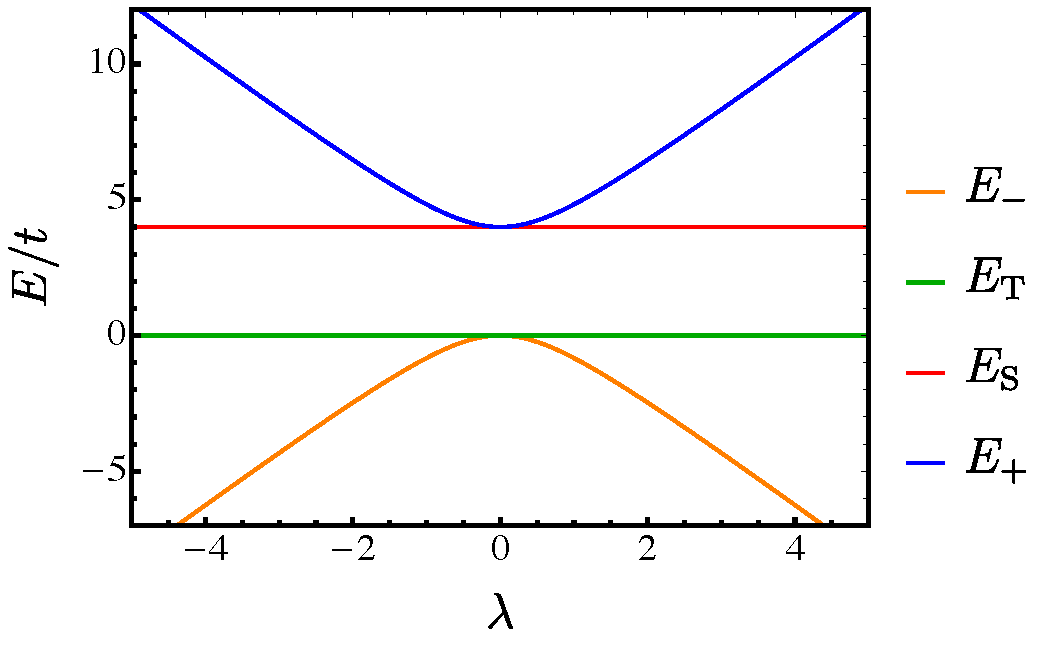
\includegraphics[height=0.65\textwidth]{fig1a}
	\subcaption{\label{subfig:FCI_real}}
    \end{subfigure}
	\begin{subfigure}{0.49\textwidth}
	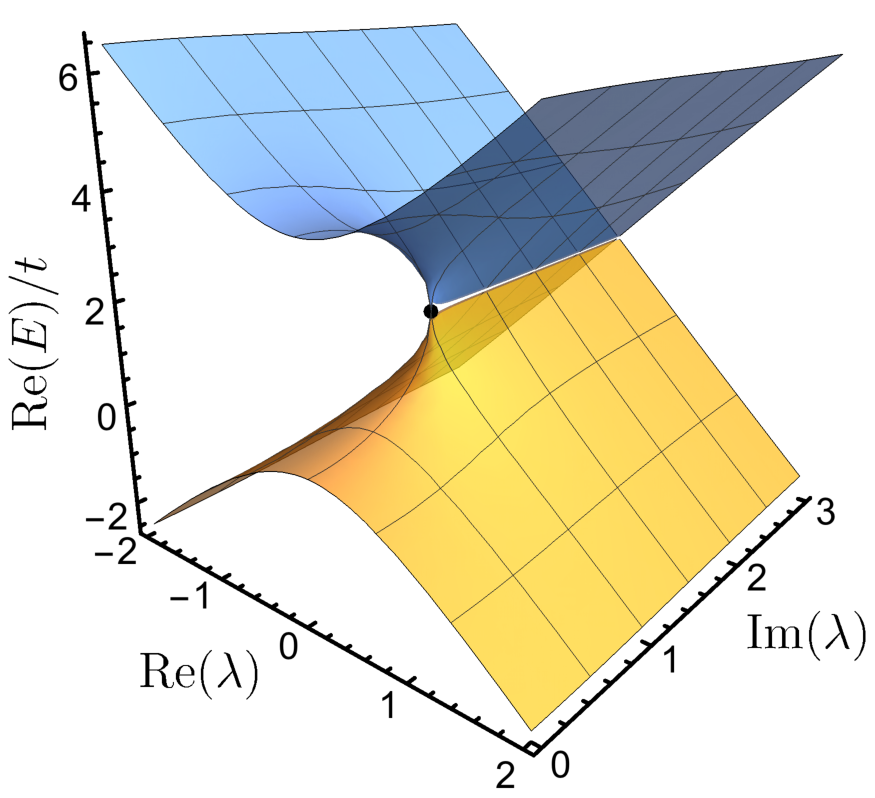
\includegraphics[height=0.65\textwidth]{fig1b}
	\subcaption{\label{subfig:FCI_cplx}}
    \end{subfigure}
	\caption{%
	Exact energies for the Hubbard dimer ($U=4t$) as functions of $\lambda$ on the real axis (\subref{subfig:FCI_real}) and in the complex plane (\subref{subfig:FCI_cplx}).
    Only the interacting closed-shell singlets are plotted in the complex plane, becoming degenerate at the EP (black dot).
    The contour followed around the EP in order to interchange states is also represented.
	\label{fig:FCI}}
\end{figure*}

To illustrate the concepts discussed throughout this article, we consider the symmetric Hubbard dimer at half filling, \ie\ with two opposite-spin fermions.
Analytically solvable models are essential in theoretical chemistry and physics as their mathematical simplicity compared to realistic systems (e.g., atoms and molecules) allows new concepts and methods to be 
easily tested while retaining the key physical phenomena.

Using the (localised) site basis, the Hilbert space of the Hubbard dimer comprises the four configurations
\begin{align*}
& \ket{\Lup \Ldown} &  & \ket{\Lup\Rdown} &  & \ket{\Rup\Ldown} &  & \ket{\Rup\Rdown}
\end{align*}
where $\Lsi$ ($\Rsi$) denotes an electron with spin $\sigma$ on the left (right) site.
The exact, or full configuration interaction (FCI), Hamiltonian is then 
\begin{equation}
\label{eq:H_FCI}
	\bH = 
	\begin{pmatrix}
		U &	- t & -  t & 0	\\
	   -  t &  0 &  0 & -  t \\
       -  t &  0 &  0 & -  t \\
        0 & -  t & -  t & U \\
	\end{pmatrix},
\end{equation}
where $t$ is the hopping parameter and $U$ is the on-site Coulomb repulsion.
We refer the interested reader to Refs.~\onlinecite{Carrascal_2015,Carrascal_2018} for more details about this system.
The parameter $U$ controls the strength of the electron correlation.
In the weak correlation regime (small $U$), the kinetic energy dominates and the electrons are delocalised over both sites.
In the large-$U$ (or strong correlation) regime, the electron repulsion term becomes dominant 
and the electrons localise on opposite sites to minimise their Coulomb repulsion. 
This phenomenon is often referred to as Wigner crystallisation. \cite{Wigner_1934}

To illustrate the formation of an EP, we scale the off-diagonal coupling strength by introducing the complex parameter $\lambda$ through the transformation $t \to \lambda t$ to give the parameterised Hamiltonian $\hH(\lambda)$.
When $\lambda$ is real, the Hamiltonian~\eqref{eq:H_FCI} is Hermitian with the distinct (real-valued) (eigen)energies
\begin{subequations}
\begin{align}
E_{\mp} &= \frac{1}{2} \qty(U \mp \sqrt{ (4 \lambda t)^2 + U^2 } ),
\label{eq:singletE}
\\
E_{\text{T}} &= 0,
\\
E_{\text{S}} &= U.
\end{align}
\end{subequations}
While the open-shell triplet ($E_{\text{T}}$) and singlet ($E_{\text{S}}$) are independent of $\lambda$, the closed-shell singlet ground state ($E_{-}$) and doubly-excited state ($E_{+}$) couple strongly to form an avoided crossing at $\lambda=0$ (see Fig.~\ref{subfig:FCI_real}).

At non-zero values of $U$ and $t$, these closed-shell singlets can only become degenerate at a pair of complex conjugate points in the complex $\lambda$ plane 
\begin{equation}
\lambda_{\text{EP}} = \pm  \i \frac{U}{4t},
\end{equation}
with energy
\begin{equation}
\label{eq:E_EP}
	E_\text{EP} = \frac{U}{2}.
\end{equation}
These $\lambda$ values correspond to so-called EPs and connect the ground and excited states in the complex plane.
Crucially, the energy surface becomes non-analytic at $\lambda_{\text{EP}}$ and a square-root singularity forms with two branch cuts running along the imaginary axis from $\lambda_{\text{EP}}$  to $\pm \i \infty$ (see Fig.~\ref{subfig:FCI_cplx}).
On the real $\lambda$ axis, these EPs lead to the singlet avoided crossing at $\lambda = \Re(\lambda_{\text{EP}})$.
The ``shape'' of this avoided crossing is related to the magnitude of $\Im(\lambda_{\text{EP}})$, with smaller values giving a ``sharper'' interaction.

Remarkably, the existence of these square-root singularities means that following a complex contour around an EP in the complex $\lambda$ plane will interconvert the closed-shell ground and excited states (see Fig.~\ref{subfig:FCI_cplx}).
This behaviour can be seen by expanding the radicand in Eq.~\eqref{eq:singletE} as a Taylor series around $\lambda_{\text{EP}}$ to give
\begin{equation}
E_{\pm} \approx E_{\text{EP}} \pm \sqrt{32t^2 \lambda_{\text{EP}}} \sqrt{\lambda - \lambda_{\text{EP}}}.
\end{equation}
Parametrising the complex contour as $\lambda(\theta) = \lambda_{\text{EP}} + R \exp(\i \theta)$ gives the continuous energy pathways 
\begin{equation}
E_{\pm} \qty(\theta) \approx E_{\text{EP}} \pm \sqrt{32t^2 \lambda_{\text{EP}} R}\, \exp(\i \theta/2)
\end{equation}
such that $E_{\pm}(2\pi)  = E_{\mp}(0)$ and $E_{\pm}(4\pi)  = E_{\pm}(0)$.
As a result, completely encircling an EP leads to the interconversion of the two interacting states, while a second complete rotation returns the two states to their original energies.
Additionally, the wave functions pick up a geometric phase in the process, and four complete loops are required to recover their starting forms.\cite{MoiseyevBook}

% LOCATING EPS
To locate EPs in practice, one must simultaneously solve
\begin{subequations}
\begin{align}
	\label{eq:PolChar}
	\det[E\hI-\hH(\lambda)] & = 0,
	\\ 
	\label{eq:DPolChar}
	\pdv{E}\det[E\hI-\hH(\lambda)] & = 0,
\end{align}
\end{subequations}
where $\hI$ is the identity operator.\cite{Cejnar_2007}
Equation \eqref{eq:PolChar} is the well-known secular equation providing the (eigen)energies of the system. 
If the energy is also solution of Eq.~\eqref{eq:DPolChar}, then this energy value is at least two-fold degenerate. 
These degeneracies can be conical intersections between two states with different symmetries 
for real values of $\lambda$,\cite{Yarkony_1996} or EPs between two states with the 
same symmetry for complex values of $\lambda$.


%============================================================%
\subsection{Rayleigh-Schr\"odinger Perturbation Theory}
%============================================================%

One of the most common routes to approximately solving the Schr\"odinger equation
is to introduce a perturbative expansion of the exact energy.
% SUMMARY OF RS-PT
Within Rayleigh-Schr\"odinger perturbation theory, the time-independent Schr\"odinger equation 
is recast as 
\begin{equation} 
	\hH(\lambda) \Psi(\lambda) 
    = \qty(\hH^{(0)} + \lambda \hV ) \Psi(\lambda) 
    = E(\lambda) \Psi(\lambda),
    \label{eq:SchrEq-PT}
\end{equation}
where $\hH^{(0)}$ is a zeroth-order Hamiltonian and $\hV = \hH - \hH^{(0)}$ represents the perturbation operator.
Expanding the wave function and energy as power series in $\lambda$ as 
\begin{subequations}
\begin{align}
    \Psi(\lambda) &= \sum_{k=0}^{\infty} \lambda^{k}\,\Psi^{(k)} 
    \label{eq:psi_expansion}
    \\
    E(\lambda) &= \sum_{k=0}^{\infty} \lambda^{k}\,E^{(k)},
    \label{eq:E_expansion}
\end{align}
\end{subequations}
solving the corresponding perturbation equations up to a given order $k$, and
setting $\lambda = 1$ then yields approximate solutions to Eq.~\eqref{eq:SchrEq}.

% MATHEMATICAL REPRESENTATION
Mathematically, Eq.~\eqref{eq:E_expansion} corresponds to a Taylor series expansion of the exact energy
around the reference system $\lambda = 0$.
The energy of the target ``physical'' system is recovered at the point $\lambda = 1$.
However, like all series expansions, Eq.~\eqref{eq:E_expansion} has a radius of convergence $\rc$. 
When $\rc < 1$, the Rayleigh--Schr\"{o}dinger expansion will diverge
for the physical system.
The value of $\rc$ can vary significantly between different systems and strongly depends on the particular decomposition
of the reference and perturbation Hamiltonians in Eq.~\eqref{eq:SchrEq-PT}.\cite{Mihalka_2017b}

% LAMBDA IN THE COMPLEX PLANE
From complex-analysis, \cite{BenderBook} the radius of convergence for the energy can be obtained by looking for the 
singularities of $E(\lambda)$ in the complex $\lambda$ plane.
This property arises from the following theorem: \cite{Goodson_2011}
\begin{quote}
\it
``The Taylor series about a point $z_0$ of a function over the complex $z$ plane will converge at a value $z_1$ 
if the function is non-singular at all values of $z$ in the circular region centred at $z_0$ with radius $\abs{z_1-z_0}$. 
If the function has a singular point $z_s$ such that $\abs{z_s-z_0} < \abs{z_1-z_0}$, 
then the series will diverge when evaluated at $z_1$.''
\end{quote}
As a result, the radius of convergence for a function is equal to the distance from the origin of the closest singularity
in the complex plane.
For example, the simple function
\begin{equation} \label{eq:DivExample}
	f(x)=\frac{1}{1+x^4}.
\end{equation}
is smooth and infinitely differentiable for $x \in \mathbb{R}$, and one might expect that its Taylor series expansion would 
converge in this domain.
However, this series diverges for $x \ge 1$.
This divergence occurs because $f(x)$ has four singularities in the complex 
($\e^{\i\pi/4}$, $\e^{-\i\pi/4}$, $\e^{\i3\pi/4}$, and $\e^{-\i3\pi/4}$) with a modulus equal to $1$, demonstrating
that complex singularities are essential to fully understand the series convergence on the real axis.\cite{BenderBook}

The radius of convergence for the perturbation series Eq.~\eqref{eq:E_expansion} is therefore dictated by the magnitude $r_c = \abs{\lambda_c}$ of the
singularity in $E(\lambda)$ that is closest to the origin.
Note that when $\abs{\lambda} = r_c$, one cannot \textit{a priori} predict if the series is convergent or not.
For example, the series $\sum_{k=1}^\infty \lambda^k/k$ diverges at $\lambda = 1$ but converges at $\lambda = -1$.

Like the exact system in Sec.~\ref{sec:example}, the perturbation energy $E(\lambda)$ represents
a ``one-to-many'' function with the output elements representing an approximation to both the ground and excited states.
The most common singularities on $E(\lambda)$ therefore correspond to non-analytic EPs in the complex 
$\lambda$ plane where two states become degenerate.
Later we will demonstrate how the choice of reference Hamiltonian controls the position of these EPs, and 
ultimately determines the convergence properties of the perturbation series.

%===========================================%
\subsection{Hartree--Fock Theory}
\label{sec:HF}
%===========================================%

% SUMMARY OF HF
In the Hartree--Fock (HF) approximation, the many-electron wave function is approximated as a single Slater determinant $\Psi^{\text{HF}}(\vb{x}_1,\ldots,\vb{x}_N)$, where $\vb{x} = (\sigma,\vb{r})$ is a composite vector gathering spin and spatial coordinates.
This Slater determinant is defined as an antisymmetric combination of $\Ne$ (real-valued) occupied one-electron spin-orbitals $\phi_p(\vb{x})$, which are, by definition, eigenfunctions of the one-electron Fock operator 
\begin{equation}\label{eq:FockOp}
    \Hat{f}(\vb{x}) \phi_p(\vb{x}) = \qty[ \Hat{h}(\vb{x}) + \Hat{v}_\text{HF}(\vb{x}) ] \phi_p(\vb{x}) = \epsilon_p \phi_p(\vb{x}).
\end{equation}
Here the (one-electron) core Hamiltonian is
\begin{equation}
\label{eq:Hcore}
	\Hat{h}(\vb{x}) = -\frac{\grad^2}{2} + \sum_{A}^{M} \frac{Z_A}{\abs{\vb{r}-\vb{R}_A}}
\end{equation}
and
\begin{equation}
    \Hat{v}_\text{HF}(\vb{x}) = \sum_i^{N} \qty[ \Hat{J}_i(\vb{x}) - \Hat{K}_i(\vb{x}) ]
\end{equation}
is the HF mean-field electron-electron potential with 
\begin{subequations}
\begin{gather}
	\label{eq:CoulOp}
    \Hat{J}_i(\vb{x})\phi_j(\vb{x})=\qty(\int \phi_i(\vb{x}')\frac{1}{\abs{\vb{r} - \vb{r}'}}\phi_i(\vb{x}') \dd\vb{x}' ) \phi_j(\vb{x}),
	\\
	\label{eq:ExcOp}
\Hat{K}_i(\vb{x})\phi_j(\vb{x})=\qty(\int \phi_i(\vb{x}')\frac{1}{\abs{\vb{r} - \vb{r}'}}\phi_j(\vb{x}') \dd\vb{x}')\phi_i(\vb{x}),
\end{gather}
\end{subequations}
defining the Coulomb and exchange operators (respectively) in the spin-orbital basis.\cite{SzaboBook}
The HF energy is then defined as 
\begin{equation}
    \label{eq:E_HF}
    E_\text{HF} = \frac{1}{2} \sum_i^{N} \qty( h_i + f_i ),
\end{equation}
with the corresponding matrix elements
\begin{align}
	h_i & = \mel{\phi_i}{\Hat{h}}{\phi_i},
    & 
    f_i & = \mel{\phi_i}{\Hat{f}}{\phi_i}.
\end{align}
The optimal HF wave function is identified by using the variational principle to minimise the HF energy.
For any system with more than one electron, the resulting Slater determinant is not an eigenfunction of the exact Hamiltonian $\hH$. 
However, it is by definition an eigenfunction of the approximate many-electron HF Hamiltonian constructed 
from the one-electron Fock operators as
\begin{equation}\label{eq:HFHamiltonian}
	\hH_{\text{HF}} = \sum_{i}^{N} f(\vb{x}_i).
\end{equation}
From hereon, $i$ and $j$ denote occupied orbitals, $a$ and $b$ denote unoccupied (or virtual) orbitals, while $p$, $q$, $r$, and $s$ denote arbitrary orbitals.

% BRIEF FLAVOURS OF HF
In the most flexible variant of real HF theory (generalised HF) the one-electron orbitals can be complex-valued
and contain a mixture of spin-up and spin-down components.\cite{Mayer_1993,Jimenez-Hoyos_2011}
However, the application of HF with some level of constraint on the orbital structure is far more common.
Forcing the spatial part of the orbitals to be the same for spin-up and spin-down electrons leads to restricted HF (RHF) method, 
while allowing different orbitals for different spins leads to the so-called unrestricted HF (UHF) approach.\cite{StuberPaldus}
The advantage of the UHF approximation is its ability to correctly describe strongly correlated systems, 
such as antiferromagnetic phases\cite{Slater_1951} or the dissociation of the hydrogen dimer.\cite{Coulson_1949}
However, by allowing different orbitals for different spins, the UHF is no longer required to be an eigenfunction of 
the total spin operator $\hat{\mathcal{S}}^2$, leading to ``spin-contamination'' in the wave function.

%================================================================%
\subsection{Hartree--Fock in the Hubbard Dimer}
\label{sec:HF_hubbard}
%================================================================%

%%% FIG 2 (?) %%%
% HF energies as a function of U/t
%%%%%%%%%%%%%%%%%
\begin{figure}
    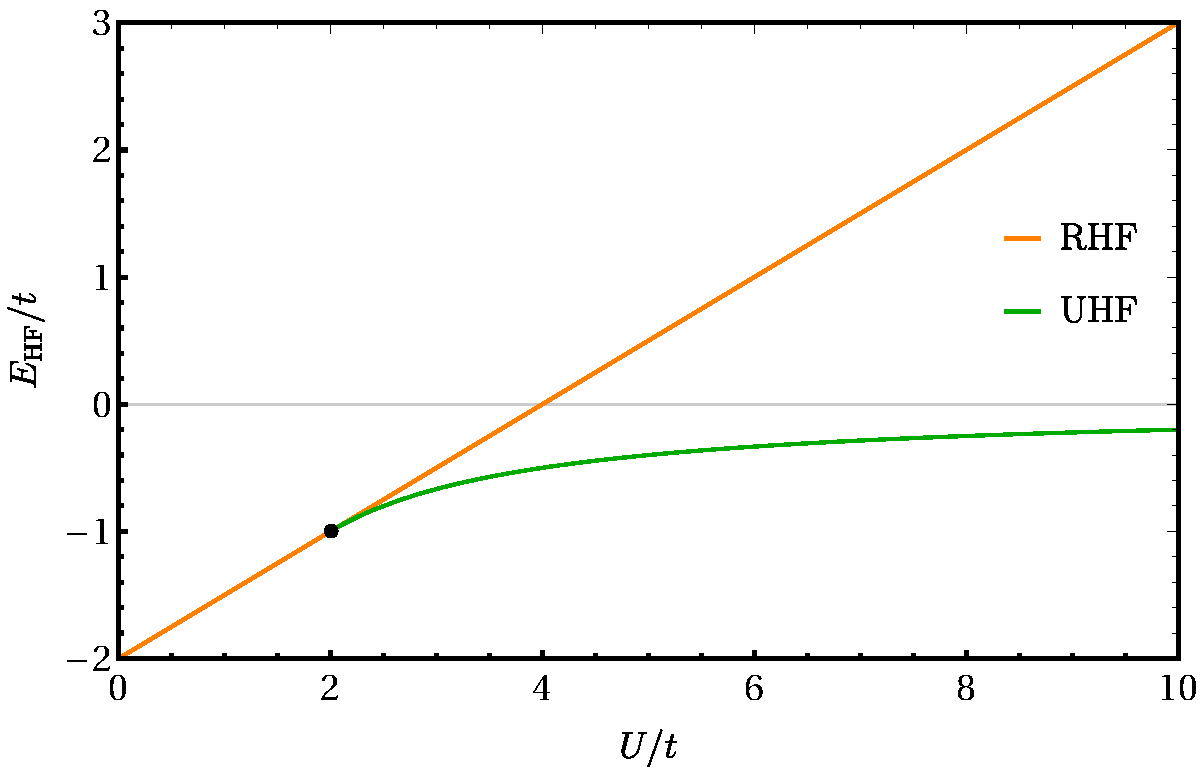
\includegraphics[width=\linewidth]{HF_real.pdf}
    \caption{\label{fig:HF_real}
    RHF and UHF energies \titou{in the Hubbard dimer} as a function of the correlation strength $U/t$. 
    The symmetry-broken UHF solution emerges at the coalescence point $U=2t$ (black dot), often known as the Coulson-Fischer point.}
\end{figure}
%%%%%%%%%%%%%%%%%

In the Hubbard dimer, the HF energy can be parametrised using two rotation angles $\ta$ and $\tb$ as
\begin{equation}
E_\text{HF}(\ta, \tb) = -t\, \qty( \sin \ta + \sin \tb ) + \frac{U}{2} \qty( 1 + \cos \ta \cos \tb ),
\end{equation}
where we have introduced bonding $\mathcal{B}^{\sigma}$ and anti-bonding $\mathcal{A}^{\sigma}$ molecular orbitals for 
the spin-$\sigma$ electrons as
\begin{subequations}
\begin{align}
    \mathcal{B}^{\sigma} & = \hphantom{-} \cos(\frac{\theta_\sigma}{2}) \Lsi + \sin(\frac{\theta_\sigma}{2}) \Rsi,
	\\
	\mathcal{A}^{\sigma} & = - \sin(\frac{\theta_\sigma}{2}) \Lsi + \cos(\frac{\theta_\sigma}{2}) \Rsi
\end{align}
\label{eq:RHF_orbs}
\end{subequations}
In the weak correlation regime $0 \le U \le 2t$, the angles which minimise the HF energy, 
\ie, $\pdv*{E_\text{HF}}{\theta_\sigma} = 0$, are 
\begin{equation}
	\ta^\text{RHF} = \tb^\text{RHF} = \pi/2,
\end{equation}
giving the symmetry-pure molecular orbitals
\begin{align}
	\mathcal{B}_\text{RHF}^{\sigma} & = \frac{\Lsi + \Rsi}{\sqrt{2}},
	&
	\mathcal{A}_\text{RHF}^{\sigma} & = \frac{\Lsi - \Rsi}{\sqrt{2}},
\end{align}
and the ground-state RHF energy (Fig.~\ref{fig:HF_real})
\begin{equation}
	E_\text{RHF} \equiv E_\text{HF}(\ta^\text{RHF}, \tb^\text{RHF}) = -2t + \frac{U}{2}
\end{equation}
However, in the strongly correlated regime $U>2t$, the closed-shell orbital restriction prevents RHF from 
modelling the correct physics with the two electrons on opposite sites.

%%% FIG 3 (?) %%%
% Analytic Continuation of HF
%%%%%%%%%%%%%%%%%
\begin{figure*}[t]
	\begin{subfigure}{0.49\textwidth}
    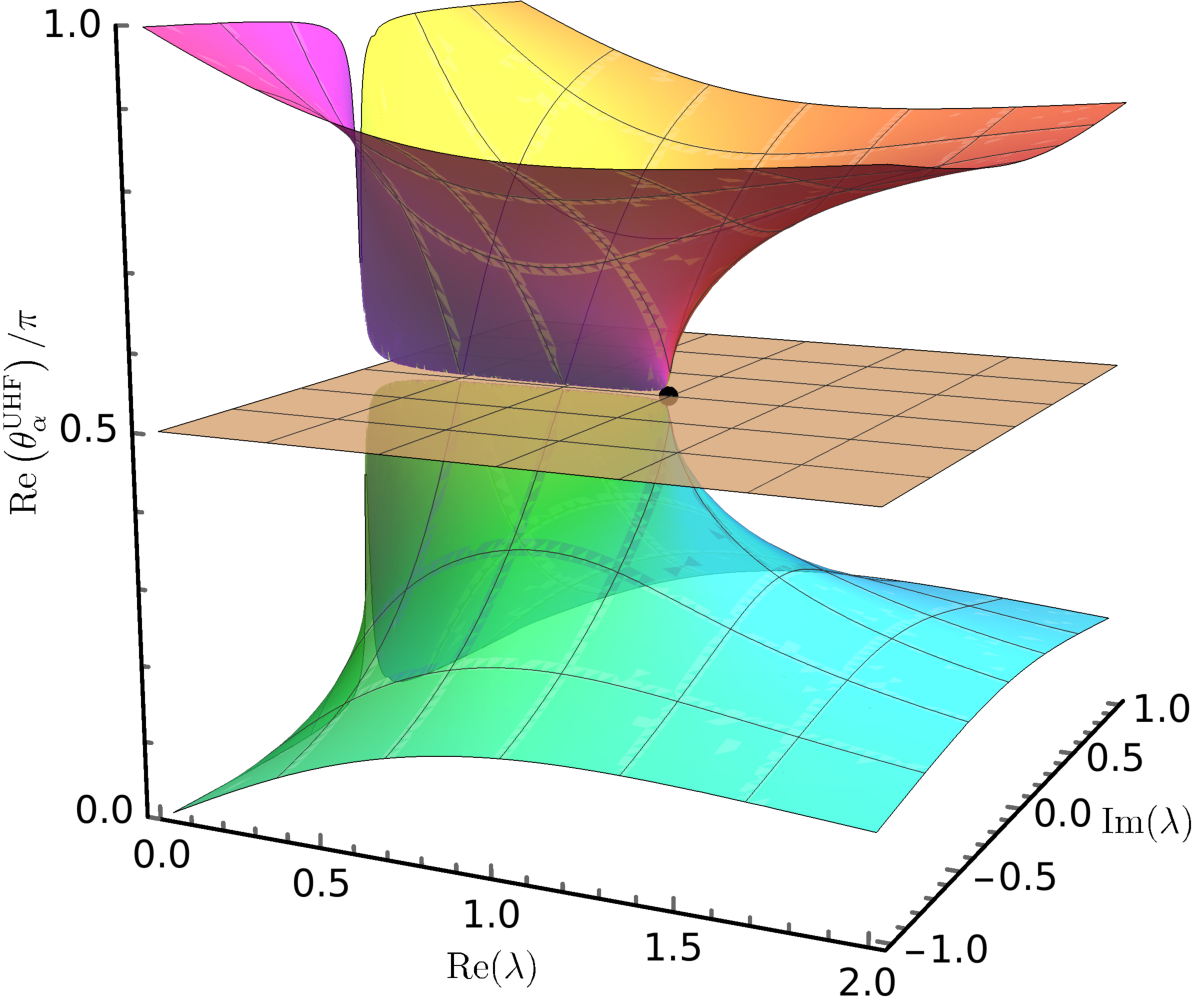
\includegraphics[height=0.65\textwidth,trim={0pt 0pt 0pt -35pt},clip]{HF_cplx_angle}
	\subcaption{\label{subfig:UHF_cplx_angle}}
    \end{subfigure}
	\begin{subfigure}{0.49\textwidth}
	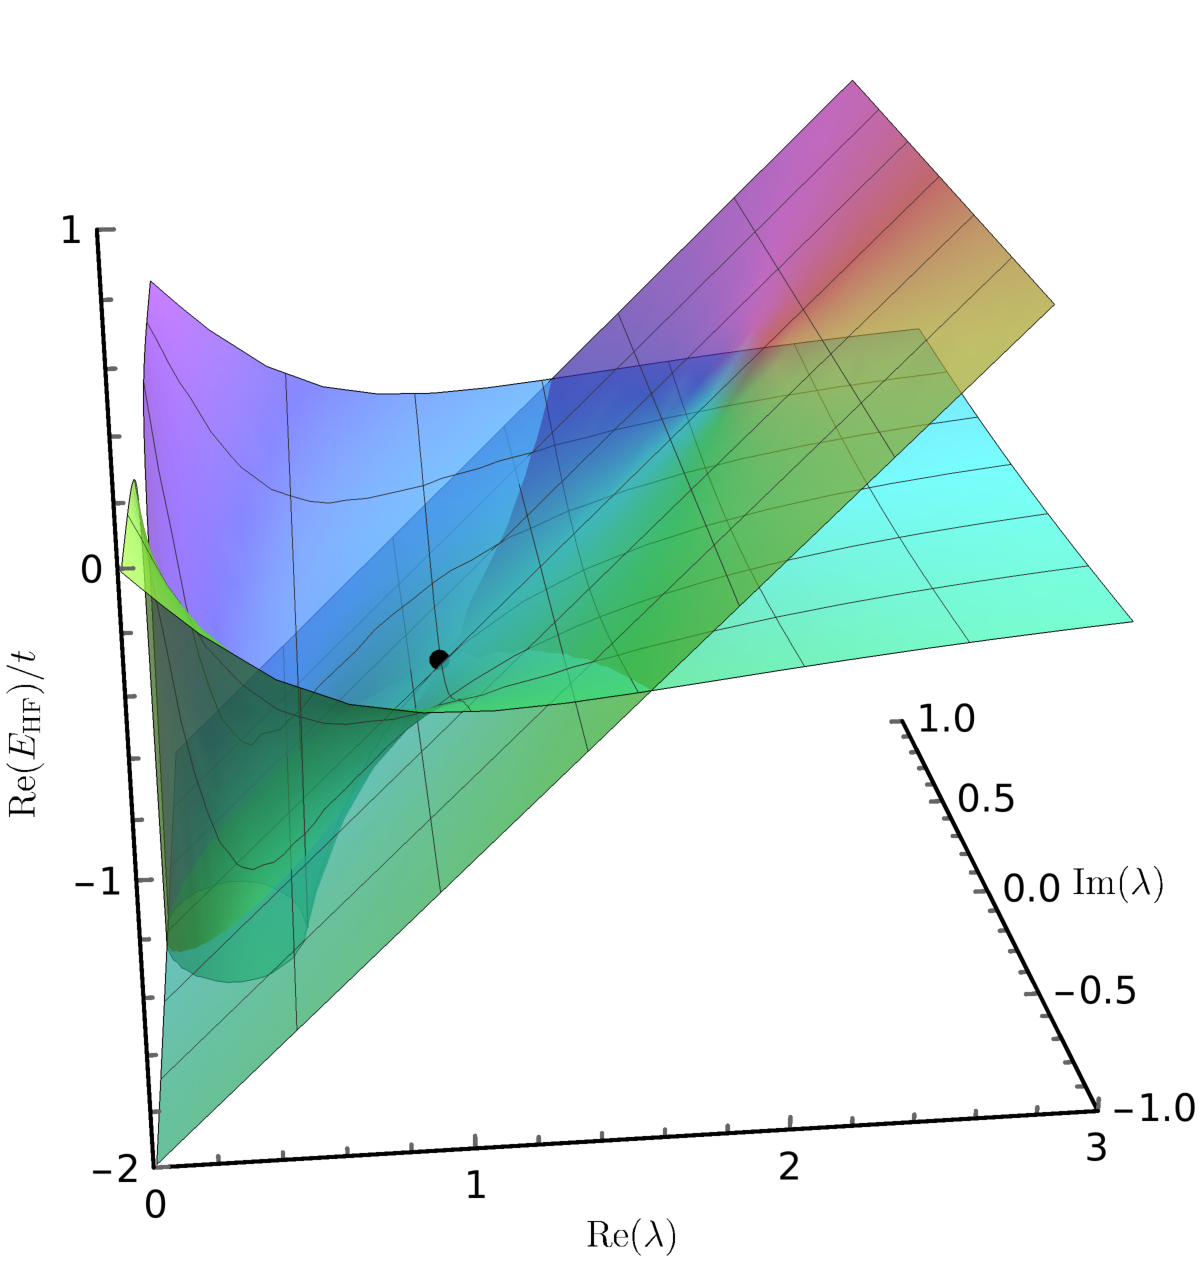
\includegraphics[height=0.65\textwidth]{HF_cplx_energy}
	\subcaption{\label{subfig:UHF_cplx_energy}}
    \end{subfigure}
	\caption{%
    (\subref{subfig:UHF_cplx_angle}) Real component of the UHF angle $\ta^{\text{UHF}}$ for $\lambda \in \bbC$ \titou{in the Hubbard dimer for $U/t = ??$}.
    Symmetry-broken solutions correspond to individual sheets and become equivalent at 
    the \textit{quasi}-EP $\lambda_{\text{c}}$ (black dot).
    The RHF solution is independent of $\lambda$, giving the constant plane at $\pi/2$.
    (\subref{subfig:UHF_cplx_energy}) The corresponding HF energy surfaces show a non-analytic 
    point at the \textit{quasi}-EP.
	\label{fig:HF_cplx}}
\end{figure*}
%%%%%%%%%%%%%%%%%

As the on-site repulsion is increased from 0, the HF approximation reaches a critical value at $U=2t$ where a symmetry-broken 
UHF solution appears with a lower energy than the RHF one.
Note that the RHF wave function remains a genuine solution of the HF equations for $U \ge 2t$, but corresponds to a saddle point 
of the HF energy rather than a minimum.
This critical point is analogous to the infamous Coulson--Fischer point identified in the hydrogen dimer.\cite{Coulson_1949}
For $U \ge 2t$, the optimal orbital rotation angles for the UHF orbitals become
\begin{subequations}
\begin{align}
    \ta^\text{UHF} & = \arctan (-\frac{2t}{\sqrt{U^2 - 4t^2}}),
    \label{eq:ta_uhf}
	\\
    \tb^\text{UHF} & = \arctan (+\frac{2t}{\sqrt{U^2 - 4t^2}}),
    \label{eq:tb_uhf}
\end{align}
\end{subequations}
with the corresponding UHF ground-state energy (Fig.~\ref{fig:HF_real})
\begin{equation}
	E_\text{UHF} \equiv E_\text{HF}(\ta^\text{UHF}, \tb^\text{UHF}) = - \frac{2t^2}{U}.
\end{equation}
Time-reversal symmetry dictates that this UHF wave function must be degenerate with its spin-flipped pair, obtained 
by swapping $\ta^{\text{UHF}}$ and $\tb^{\text{UHF}}$ in Eqs.~\eqref{eq:ta_uhf} and \eqref{eq:tb_uhf}.
This type of symmetry breaking is also called a spin-density wave in the physics community as the system
``oscillates'' between the two symmetry-broken configurations. \cite{GiulianiBook}
Symmetry breaking can also occur in RHF theory when a charge-density wave is formed from an oscillation 
between the two closed-shell configurations with both electrons localised on one site or the other.\cite{StuberPaldus,Fukutome_1981}

%============================================================%
\subsection{Self-Consistency as a Perturbation} %OR {Complex adiabatic connection}
%============================================================%

% INTRODUCE PARAMETRISED FOCK HAMILTONIAN
The inherent non-linearity in the Fock eigenvalue problem arises from self-consistency 
in the HF approximation, and is usually solved through an iterative approach.\cite{Roothaan_1951,Hall_1951}
Alternatively, the non-linear terms arising from the Coulomb and exchange operators can 
be considered as a perturbation from the core Hamiltonian \eqref{eq:Hcore} by introducing the
transformation $U \to \lambda\, U$, giving the parametrised Fock operator 
\begin{equation}
    \Hat{f}(\vb{x} ; \lambda) = \Hat{h}(\vb{x}) + \lambda\, \Hat{v}_\text{HF}(\vb{x}).
\end{equation}
The orbitals in the reference problem $\lambda=0$ correspond to the symmetry-pure eigenfunctions of the one-electron core
Hamiltonian, while self-consistent solutions at $\lambda = 1$ represent the orbitals of the true HF solution.

% INTRODUCE COMPLEX ANALYTIC-CONTINUATION
For real $\lambda$, the self-consistent HF energies at given (real) $U$ and $t$ values
in the Hubbard dimer directly mirror the energies shown in Fig.~\ref{fig:HF_real}, 
with coalesence points at 
\begin{equation}
    \lambda_{\text{c}} = \pm \frac{2t}{U}.
    \label{eq:scaled_fock}
\end{equation}
In contrast, when $\lambda$ becomes complex, the HF equations become non-Hermitian and 
each HF solutions can be analytically continued for all $\lambda$ values using
the holomorphic HF approach.\cite{Hiscock_2014,Burton_2016,Burton_2018}
Remarkably, the coalescence point in this analytic continuation emerges as a 
\textit{quasi}-EP on the real $\lambda$ axis (Fig.~\ref{fig:HF_cplx}), where
the different HF solutions become equivalent but not self-orthogonal.\cite{Burton_2019}
By analogy with perturbation theory, the regime where this \textit{quasi}-EP occurs 
within $\lambda_{\text{c}} \le 1$ can be interpreted as an indication that 
the symmetry-pure reference orbitals no longer provide a qualitatively 
accurate representation for the true HF ground state at $\lambda = 1$.
For example, in the Hubbard dimer with $U > 2t$, one finds $\lambda_{\text{c}} < 1$ and the symmetry-pure orbitals
do not provide a good representation of the HF ground state.
In contrast, $U < 2t$ yields $\lambda_{\text{c}} > 1$ and corresponds to
the regime where the HF ground state is correctly represented by symmetry-pure orbitals.

% COMPLEX ADIABATIC CONNECTION
We have recently shown that the complex scaled Fock operator \eqref{eq:scaled_fock}
also allows states of different symmetries to be interconverted by following a well-defined
contour in the complex $\lambda$-plane.\cite{Burton_2019}
In particular, by slowly varying $\lambda$ in a similar (yet different) manner
to an adiabatic connection in density-functional theory,\cite{Langreth_1975,Gunnarsson_1976,Zhang_2004} 
a ground-state wave function can be ``morphed'' into an excited-state wave function 
via a stationary path of HF solutions.
This novel approach to identifying excited-state wave functions demonstrates the fundamental 
role of \textit{quasi}-EPs in determining the behaviour of the HF approximation.

%%%%%%%%%%%%%%%%%%%%%%%%%%%%%%%%%%%%%%%%%%%%%%%
\section{M{\o}ller--Plesset Perturbation Theory in the Complex Plane}
\label{sec:MP}
%%%%%%%%%%%%%%%%%%%%%%%%%%%%%%%%%%%%%%%%%%%%%%%

%=====================================================%
\subsection{Background Theory}
%=====================================================%

In electronic structure, the HF Hamiltonian \eqref{eq:HFHamiltonian} is often used as the zeroth-order Hamiltonian
to define M\o{}ller--Plesset (MP) perturbation theory.\cite{Moller_1934}
This approach can recover a large proportion of the electron correlation energy,\cite{Lowdin_1955a,Lowdin_1955b,Lowdin_1955c} 
and provides the foundation for numerous post-HF approximations.
With the MP partitioning, the parametrised perturbation Hamiltonian becomes
\begin{multline}\label{eq:MPHamiltonian}
    \hH(\lambda) =   
     \sum_{i}^{N} \qty[ - \frac{\grad_i^2}{2} - \sum_{A}^{M} \frac{Z_A}{\abs{\vb{r}_i-\vb{R}_A}} ]
    \\
    + (1-\lambda) \sum_{i}^{N} v^{\text{HF}}(\vb{x}_i)
    + \lambda\sum_{i<j}^{N}\frac{1}{\abs{\vb{r}_i-\vb{r}_j}}.
\end{multline}
Any set of orbitals can be used to define the HF Hamiltonian, although either the RHF or UHF orbitals are usually chosen to 
define the RMP or UMP series respectively.
The MP energy at a given order $n$ (\ie, MP$n$) is then defined as
\begin{equation}
	E_{\text{MP}n}= \sum_{k=0}^n E_{\text{MP}}^{(k)},
\end{equation}
where $E_{\text{MP}}^{(k)}$ is the $k$th-order MP correction and 
\begin{equation}
E_{\text{MP1}} =  E_{\text{MP}}^{(0)} + E_{\text{MP}}^{(1)} = E_\text{HF}.
\end{equation}
The second-order MP2 energy is given by
\begin{equation}\label{eq:EMP2}
	E_{\text{MP2}} = \frac{1}{4} \sum_{ij} \sum_{ab} \frac{\abs{\mel{ij}{}{ab}}^2}{\epsilon_i + \epsilon_j - \epsilon_a - \epsilon_b},
\end{equation}
where $\mel{pq}{}{rs} = \braket{pq}{rs} - \braket{pq}{sr}$ are the anti-symmetrised two-electron integrals
in the molecular spin-orbital basis\cite{Gill_1994}
\begin{equation}
	\braket{pq}{rs} 
    = \iint \dd\vb{x}_1\dd\vb{x}_2
    \frac{\phi^{*}_p(\vb{x}_1)\phi^{*}_q(\vb{x}_2)\phi^{\vphantom{*}}_r(\vb{x}_1)\phi^{\vphantom{*}}_s(\vb{x}_2)}%
      {\abs{\vb{r}_1 - \vb{r}_2}}.
\end{equation}

While most practical calculations generally consider only the MP2 or MP3 approximations, higher order terms can 
easily be computed to understand the convergence of the MP$n$ series.\cite{Handy_1985}
\textit{A priori}, there is no guarantee that this series will provide the smooth convergence that is desirable for a
systematically improvable theory.
In fact, when the reference HF wave function is a poor approximation to the exact wave function, 
for example in multi-configurational systems, MP theory can yield highly oscillatory, 
slowly convergent, or catastrophically divergent results.\cite{Gill_1986,Gill_1988,Handy_1985,Lepetit_1988,Leininger_2000}
Furthermore, the convergence properties of the MP series can depend strongly on the choice of restricted or
unrestricted reference orbitals.

Although practically convenient for electronic structure calculations, the MP partitioning is not 
the only possibility and alternative partitionings have been considered including: 
i) the Epstein-Nesbet (EN) partitioning which consists in taking the diagonal elements of $\hH$ as the zeroth-order Hamiltonian. \cite{Nesbet_1955,Epstein_1926} 
ii) the weak correlation partitioning in which the one-electron part is consider as the unperturbed Hamiltonian $\hH^{(0)}$ and the two-electron part is the perturbation operator $\hV$, and 
iii) the strong coupling partitioning where the two operators are inverted compared to the weak correlation partitioning. \cite{Seidl_2018}
While an in-depth comparison of these different approaches can offer insight into 
their relative strengths and weaknesses for various situations, we will restrict our current discussion
to the convergence properties of the MP expansion.

%=====================================================%
\subsection{Early Studies of M{\o}ller--Plesset Convergence} % in Molecular Systems}
%=====================================================%

% GENERAL DESIRE FOR WELL-BEHAVED CONVERGENCE AND LOW-ORDER TERMS
Among the most desirable properties of any electronic structure technique is the existence of 
a systematic route to increasingly accurate energies. 
In the context of MP theory, one would like a monotonic convergence of the perturbation
series towards the exact energy such that the accuracy increases as each term in the series is added.
If such well-behaved convergence can be established, then our ability to compute individual 
terms in the series becomes the only barrier to computing the exact correlation in a finite basis set.
Unfortunately, the computational scaling of each term in the MP series increases with the perturbation
order, and practical calculations must rely on fast convergence
to obtain high-accuracy results using only the lowest order terms.

% INITIAL POSITIVITY AROUND THE CONVERGENCE PROPERTIES AND EARLY WORK SCOPE
MP theory was first introduced to quantum chemistry through the pioneering
works of Bartlett \etal\ in the context of many-body perturbation theory,\cite{Bartlett_1975}
and Pople and co-workers in the context of determinantal expansions.\cite{Pople_1976,Pople_1978}
Early implementations were restricted to the fourth-order MP4 approach that was considered
to offer state-of-the-art quantitative accuracy.\cite{Pople_1978,Krishnan_1980}
However, it was quickly realised that the MP series often demonstrated very slow, oscillatory, 
or erratic convergence, with the UMP series showing particularly slow convergence.\cite{Laidig_1985,Knowles_1985,Handy_1985}
For example, RMP5 is worse than RMP4 for predicting the homolytic barrier fission of \ce{He2^2+} using a minimal basis set, 
while the UMP series monotonically converges but becomes increasingly slow beyond UMP5.\cite{Gill_1986}
The first examples of divergent MP series were observed in the \ce{N2} and \ce{F2} 
diatomics, where low-order RMP and UMP expansions give qualitatively wrong binding curves.\cite{Laidig_1987} 

% SLOW UMP CONVERGENCE AND SPIN CONTAMINATION
The divergence of RMP expansions for stretched bonds can be easily understood from two perspectives.\cite{Gill_1988a}
Firstly, the exact wave function becomes increasingly multi-configurational as the bond is stretched, and the 
\titou{R}HF wave function no longer provides a qualitatively correct reference for the perturbation expansion.
Secondly, the energy gap between the bonding and antibonding orbitals associated with the stretch becomes
increasingly small at larger bond lengths, \titou{leading to a divergence, for example, in the second-order MP correction \eqref{eq:EMP2}.}
In contrast, the origin of slow UMP convergence is less obvious as the reference UHF energy remains
qualitatively correct at large bond lengths and the orbital degeneracy is avoided.
Furthermore, this slow convergence can also be observed in molecules with a UHF ground state at the equilibrium
geometry (\eg, \ce{CN-}), suggesting a more fundamental link with spin-contamination 
in the reference wave function.\cite{Nobes_1987}

Using the UHF framework allows the singlet ground state wave function to mix with triplet wave functions, 
leading to spin contamination where the wave function is no longer an eigenfunction of the $\Hat{\cS}^2$ operator.
The link between slow UMP convergence and this spin-contamination was first systematically investigated
by Gill \etal\ using the minimal basis \ce{H2} model.\cite{Gill_1988}
In this work, the authors compared \titou{the UMP series with the exact RHF- and UHF-based FCI expansions (T2: I don't understand this)}
and identified that the slow UMP convergence arises from its failure to correctly predict the amplitude of the
low-lying double excitation.
This erroneous description of the double excitation amplitude has the same origin as the spin-contamination in the reference
UHF wave function, creating the first direct link between spin-contamination and slow UMP convergence.\cite{Gill_1988}

% LEPETIT CHAT
Lepetit \etal\ later analysed the difference between perturbation convergence using the UMP 
and EN partitionings. \cite{Lepetit_1988}
They argued that the slow UMP convergence for stretched molecules arises from 
(i) the fact that the MP denominator (see Eq.~\ref{eq:EMP2})
tends to a constant value instead of vanishing, and (ii) the slow convergence of contributions from the 
singly-excited configurations that strongly couple to the doubly-excited configurations and first
appear at fourth-order.\cite{Lepetit_1988}
Drawing these ideas together, we believe that slow UMP convergence occurs because the single excitations must focus on removing
spin-contamination from the reference wave function, limiting their ability to fine-tune the amplitudes of the higher 
excitations that capture the correlation energy.

% SPIN-PROJECTION SCHEMES
A number of spin-projected extensions have been derived to reduce spin-contamination in the wave function
and overcome the slow UMP convergence.
Early versions of these theories, introduced by Schlegel \cite{Schlegel_1986, Schlegel_1988} or 
Knowles and Handy,\cite{Knowles_1988a,Knowles_1988b} exploited the ``projection-after-variation'' philosophy,
where the spin-projection is applied directly to the UMP expansion.
These methods succeeded in accelerating the convergence of the projected MP series and were 
considered as highly effective methods for capturing the electron correlation at low computational cost.\cite{Knowles_1988b}
However, the use of projection-after-variation leads to gradient discontinuities in the vicinity of the UHF symmetry-breaking point,
and can result in spurious minima along a molecular binding curve.\cite{Schlegel_1986,Knowles_1988a}
More recent formulations of spin-projected perturbations theories have considered the  
``variation-after-projection'' framework using alternative definitions of the reference 
Hamiltonian.\cite{Tsuchimochi_2014,Tsuchimochi_2019}
These methods yield more accurate spin-pure energies without 
gradient discontinuities or spurious minima.

%==========================================%
\subsection{Spin-Contamination in the Hubbard Dimer}
\label{sec:spin_cont}
%==========================================%

%%% FIG 2 %%%
\begin{figure*}
	\begin{subfigure}{0.32\textwidth}
	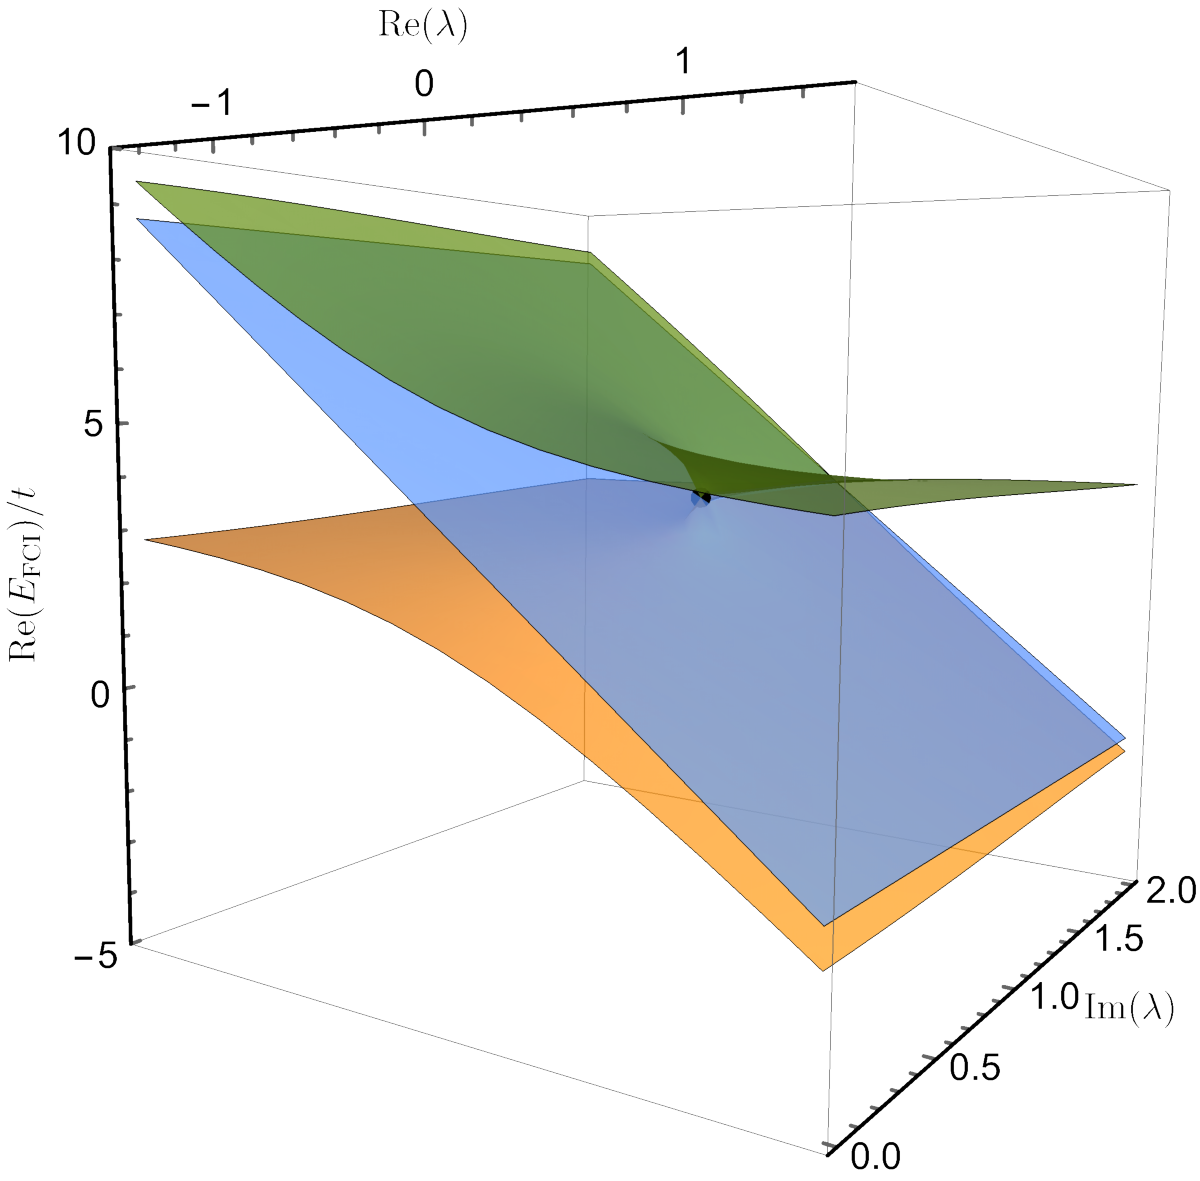
\includegraphics[height=0.75\textwidth]{fig2a}	
		\subcaption{\label{subfig:RMP_3.5} $U/t = 3.5$}
    \end{subfigure}
    %
    \begin{subfigure}{0.32\textwidth}
	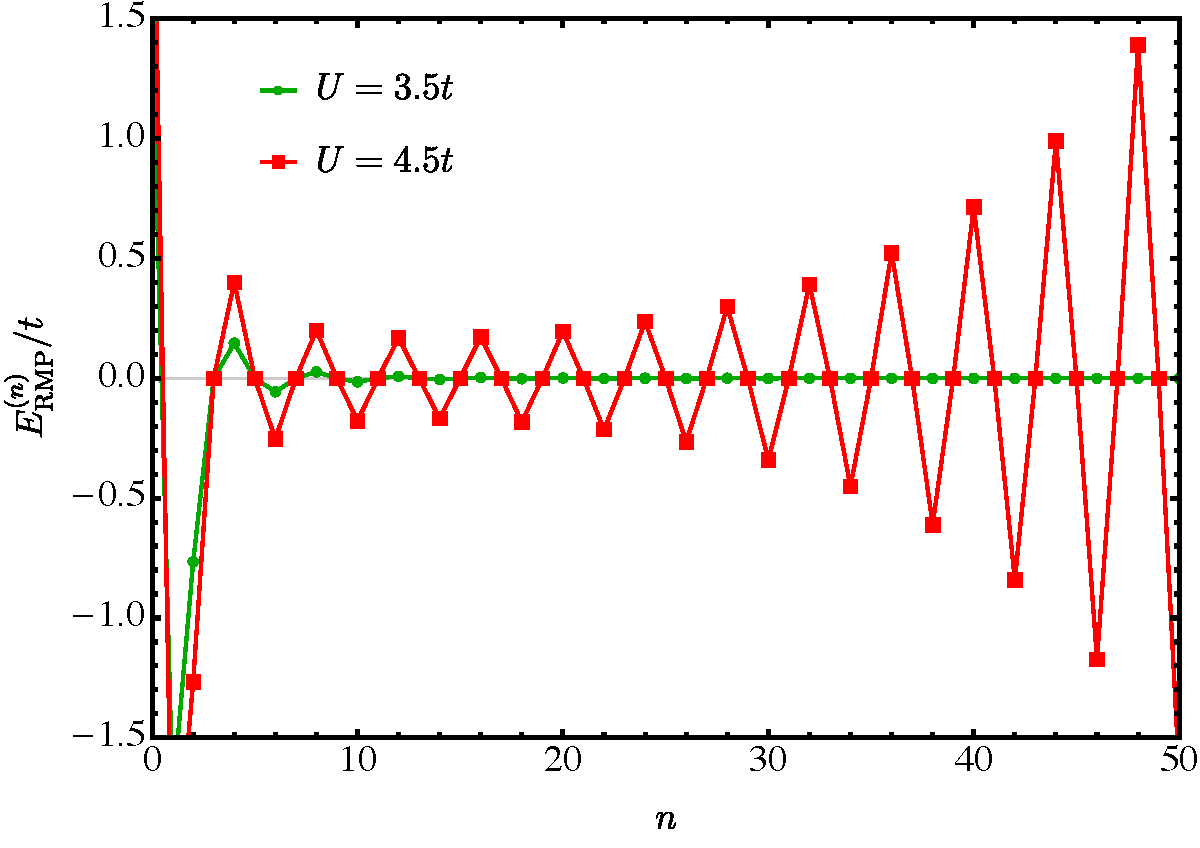
\includegraphics[height=0.75\textwidth]{fig2b}
		\subcaption{\label{subfig:RMP_cvg}}
    \end{subfigure}
    %
    \begin{subfigure}{0.32\textwidth}
	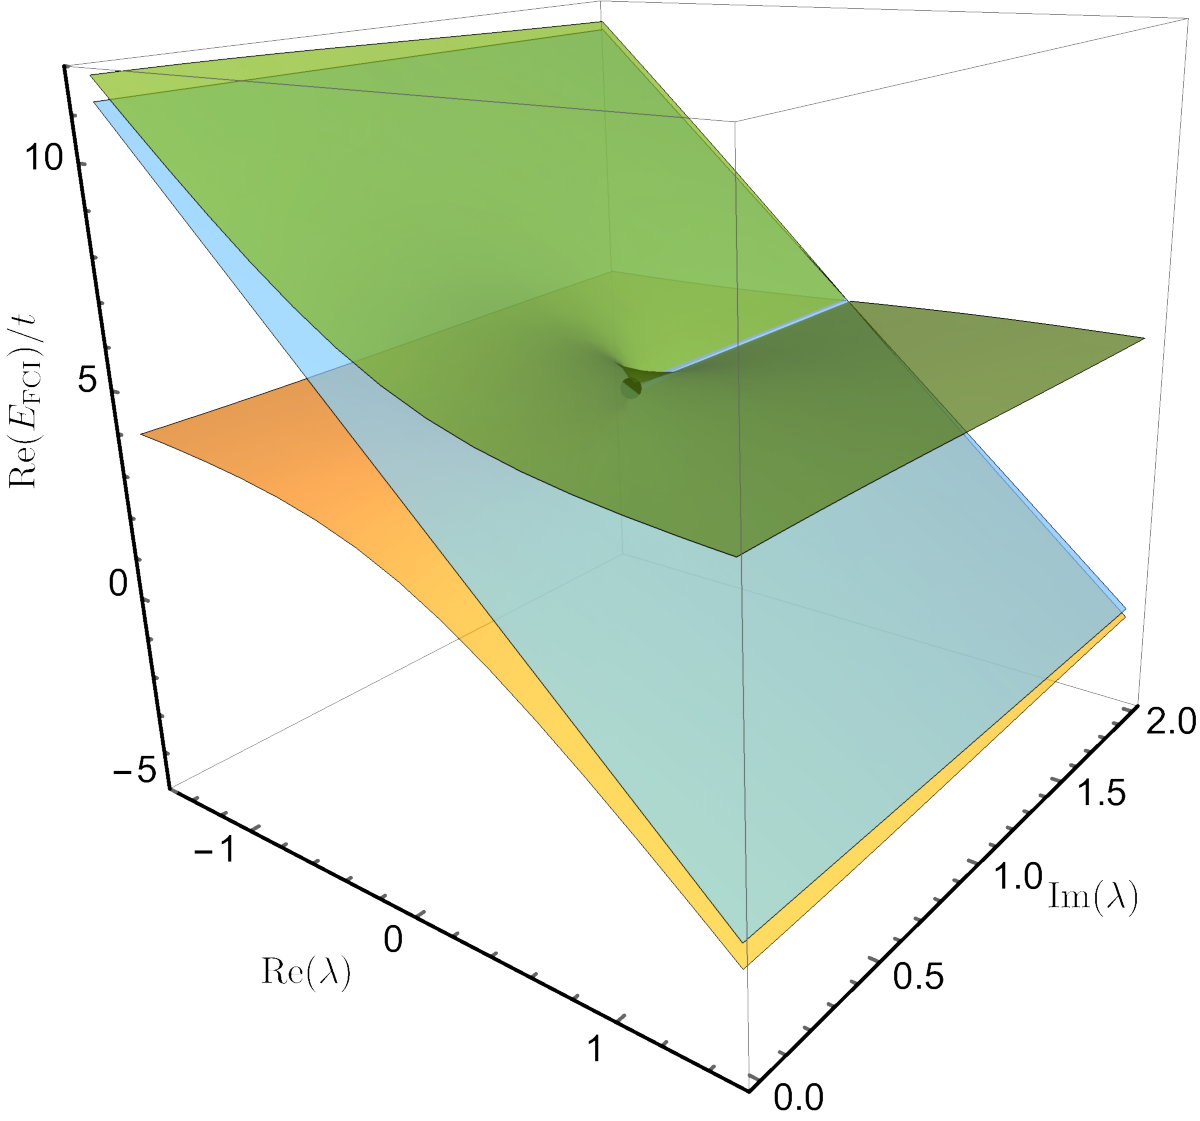
\includegraphics[height=0.75\textwidth]{fig2c}	
		\subcaption{\label{subfig:RMP_4.5} $U/t = 4.5$}
    \end{subfigure}
	\caption{
	Convergence of the RMP series as a function of the perturbation order $n$ for the Hubbard dimer at $U/t = 3.5$ (where $r_c > 1$) and $4.5$ (where $r_c < 1$).
	The Riemann surfaces associated with the exact energies of the RMP Hamiltonian \eqref{eq:H_RMP} are also represented for these two values of $U/t$ as functions of $\lambda$. 
	\label{fig:RMP}}
\end{figure*}

The behaviour of the RMP and UMP series observed in \ce{H2} can also be illustrated by considering
the analytic Hubbard dimer with a complex-valued perturbation strength.
In this system, the stretching of the \ce{H\bond{-}H} bond is directly mirrored by an increase in the \trash{electron correlation} \titou{ratio} $U/t$.
Using the ground-state RHF reference orbitals leads to the parametrised RMP Hamiltonian
\begin{widetext}
\begin{equation}
\label{eq:H_RMP}
\bH_\text{RMP}\qty(\lambda) = 
	\begin{pmatrix}
		-2t + U - \lambda U/2	&	0					&	0					&	\lambda U/2	\\
		0						&	U - \lambda U/2 	&	\lambda U/2			&	0	\\
		0						&	\lambda U/2			&	U - \lambda U/2 	&	0	\\
		\lambda U/2 			&	0 					&	0					&	2t + U - \lambda U/2	\\
	\end{pmatrix},
\end{equation}
\end{widetext}
which yields the ground-state energy 
\begin{equation}
	\label{eq:E0MP}
	E_{-}(\lambda) = U - \frac{\lambda U}{2} - \frac{1}{2} \sqrt{(4t)^2 + \lambda ^2 U^2}.
\end{equation}
From this expression, the EPs can be identified as $\lep = \pm \i 4t / U$,
giving the radius of convergence
\begin{equation}
    \rc = \abs{\frac{4t}{U}}.
\end{equation}
Remarkably, these EPs are identical to the exact EPs discussed in Sec.~\ref{sec:example}.
The Taylor expansion of the RMP energy can then be evaluated to obtain the $k$th-order MP correction
\begin{equation}
	E_\text{RMP}^{(k)} = U \delta_{0,k} - \frac{1}{2} \frac{U^k}{(4t)^{k-1}} \mqty( 1/2 \\ k/2).
\end{equation}
 
%%%%%%%%%%%%%%%%%%%%%%%%%%%%%
% RADIUS OF CONVERGENCE PLOTS
%%%%%%%%%%%%%%%%%%%%%%%%%%%%%
\begin{figure}[htb]
	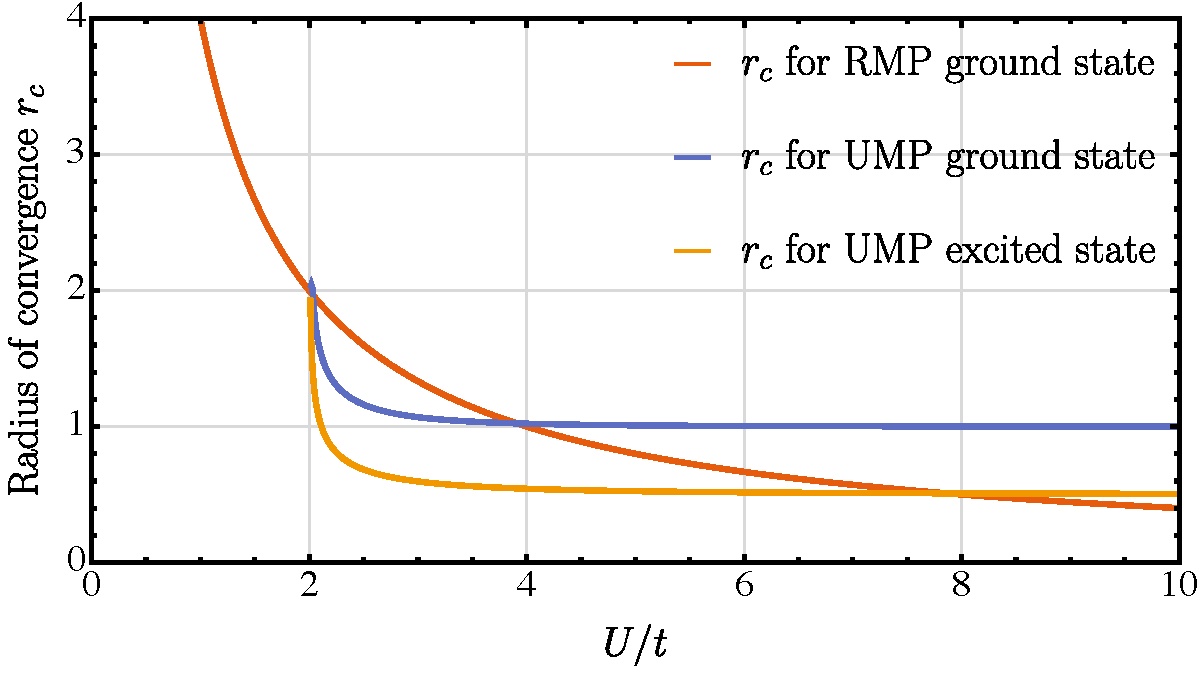
\includegraphics[width=\linewidth]{RadConv}
	\caption{
	Radius of convergence $r_c$ for the RMP ground state (red), the UMP ground state (blue), and the UMP excited state (orange) 
    series as functions of the ratio $U/t$.
	\label{fig:RadConv}}
\end{figure}
%%%%%%%%%%%%%%%%%%%%%%%%%%%%%

The RMP series is convergent for $U = 3.5\,t$ with $\rc > 1$, as illustrated for the individual terms at each order
of perturbation in Fig.~\ref{subfig:RMP_cvg}.
In contrast, for $U = 4.5t$ one finds $\rc < 1$, and the RMP series becomes divergent.
The corresponding Riemann surfaces for $U = 3.5\,t$ and $4.5\,t$ are shown in Figs.~\ref{subfig:RMP_3.5} and 
\ref{subfig:RMP_4.5}, respectively, with the single EP at $\lep$ (black dot) and the radius of convergence indicated
by the vertical cylinder of unit radius.
For the divergent case, the $\lep$ lies inside this cylinder of convergence, while in the convergent case $\lep$ lies
outside this cylinder.
In both cases, the EP connects the ground state with the doubly-excited state, and thus the convergence behaviour
for the two states using the ground-state RHF orbitals is identical.

%%% FIG 3 %%%
\begin{figure*}
	\begin{subfigure}{0.32\textwidth}
	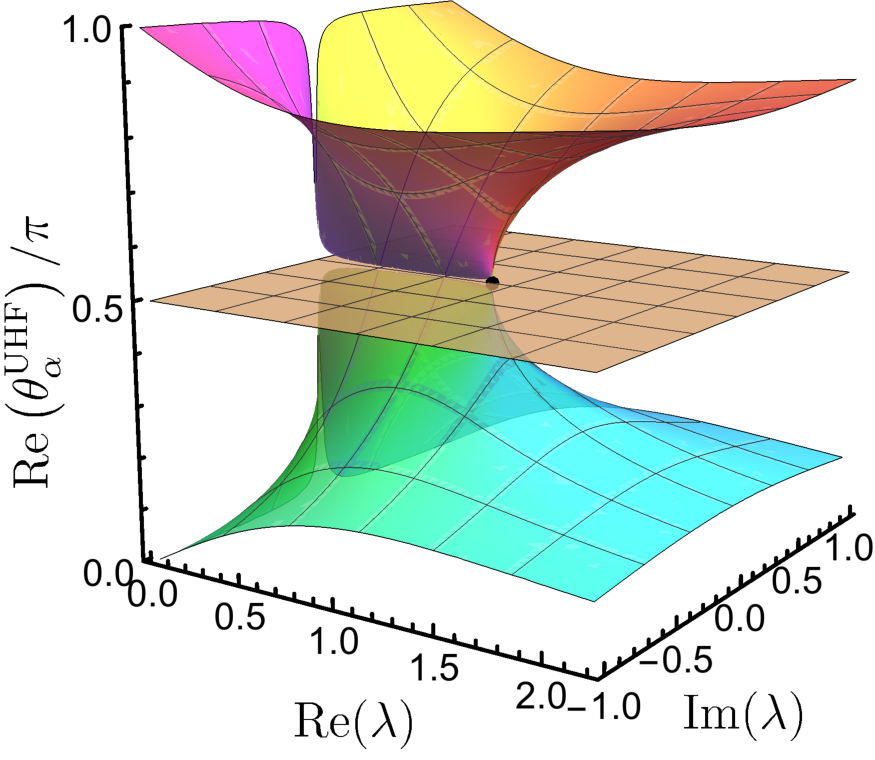
\includegraphics[height=0.75\textwidth]{fig3a}	
		\subcaption{\label{subfig:UMP_3} $U/t = 3$}
    \end{subfigure}
    %
    \begin{subfigure}{0.32\textwidth}
	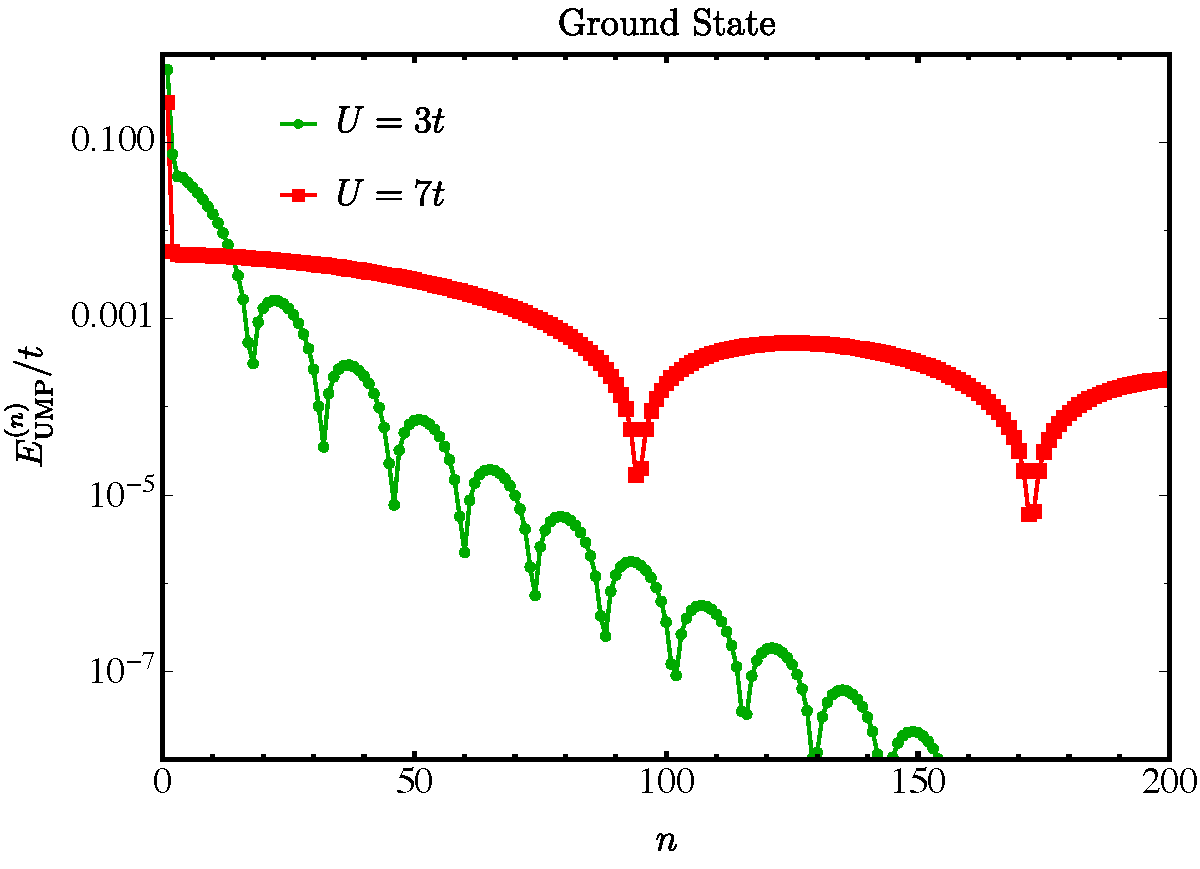
\includegraphics[height=0.75\textwidth]{fig3b}
		\subcaption{\label{subfig:UMP_cvg}}
    \end{subfigure}
    %
    \begin{subfigure}{0.32\textwidth}
	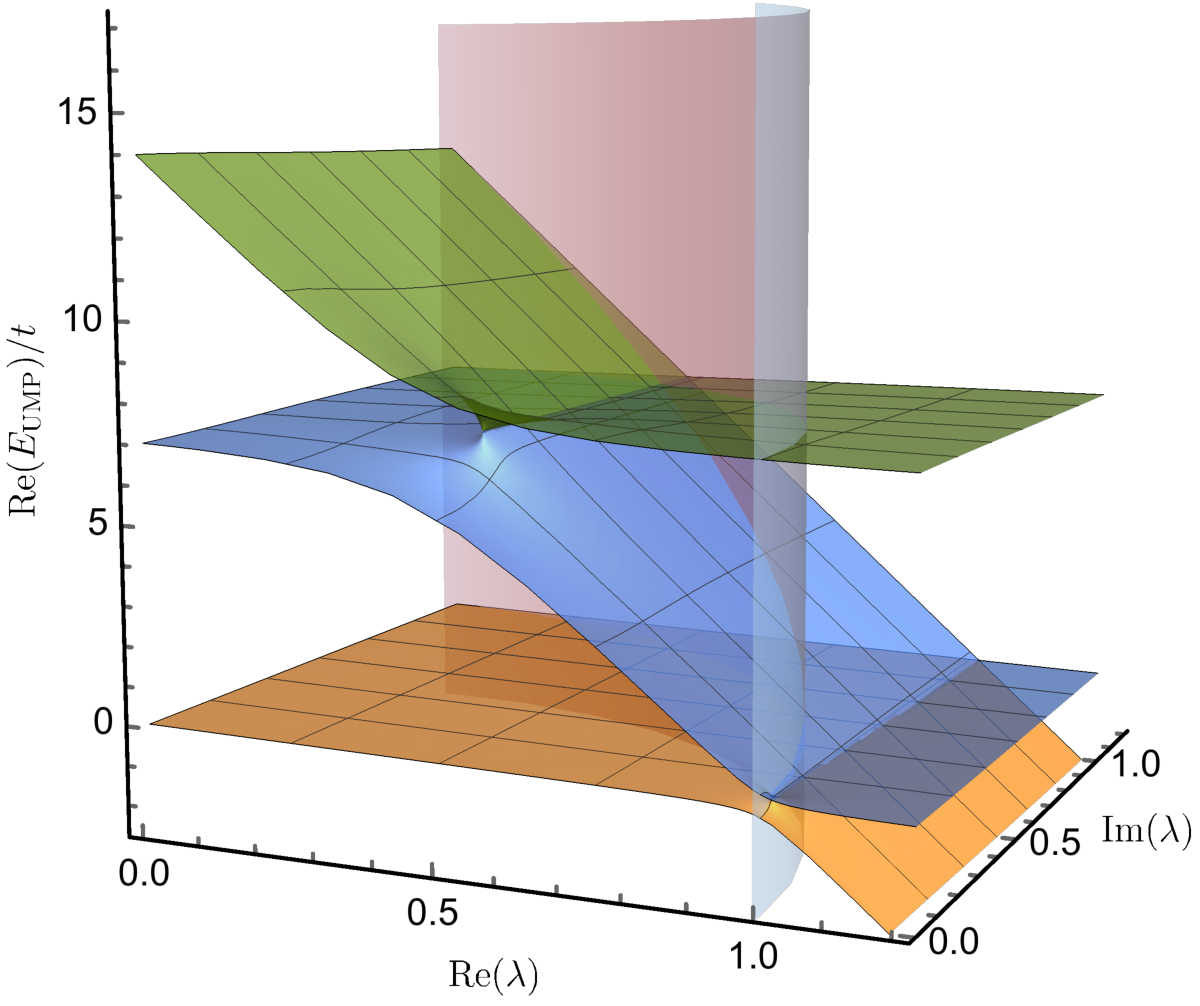
\includegraphics[height=0.75\textwidth]{fig3c}	
		\subcaption{\label{subfig:UMP_7} $U/t = 7$}
    \end{subfigure}	\caption{
	Convergence of the UMP series as a function of the perturbation order $n$ for the Hubbard dimer at $U/t = 3$ and $7$.
	The Riemann surfaces associated with the exact energies of the UMP Hamiltonian \eqref{eq:H_UMP} are also represented for these two values of $U/t$ as functions of $\lambda$.
	\label{fig:UMP}}
\end{figure*}

The behaviour of the UMP series is more subtle than the RMP series as the spin-contamination in the wave function
introduces additional coupling between the singly- and doubly-excited configurations.
Using the ground-state UHF reference orbitals in the Hubbard dimer yields the parametrised UMP Hamiltonian
\begin{widetext}
\begin{equation}
\label{eq:H_UMP}
\bH_\text{UMP}\qty(\lambda) = 
	\begin{pmatrix}
		-2t^2 \lambda/U	&	0									&	0									&	2t^2 \lambda/U		\\
		0				&	U - 2t^2 \lambda/U 					&	2t^2\lambda/U						&	2t \sqrt{U^2 - (2t)^2} \lambda/U	\\
		0				&	2t^2\lambda/U						&	U - 2t^2 \lambda/U 					&	-2t \sqrt{U^2 - (2t)^2} \lambda/U	\\
		2t^2 \lambda/U	&	2t \sqrt{U^2 - (2t)^2} \lambda/U 	&	-2t \sqrt{U^2 - (2t)^2} \lambda/U	&	2U(1-\lambda) + 6t^2\lambda/U		\\
	\end{pmatrix}.
\end{equation}
\end{widetext}
While a closed-form expression for the ground-state energy exists, it is cumbersome and we eschew reporting it.
Instead, the radius of convergence of the UMP series can be obtained numerically as a function of $U/t$, as shown
in Fig.~\ref{fig:RadConv}.
These numerical values reveal that the UMP ground-state series has $\rc > 1$ for all $U/t$ and always converges.
However, in the strong correlation limit (large $U/t$), this radius of convergence tends to unity, indicating that
the convergence of the corresponding UMP series becomes increasingly slow.
Furthermore, the doubly-excited state using the ground-state UHF orbitals has $\rc < 1$ for almost any value 
of $U/t$, reaching the limiting value of $1/2$ for $U/t \to \infty$. Hence, the 
excited-state UMP series will always diverge.
 
% DISCUSSION OF UMP RIEMANN SURFACES
The convergence behaviour can be further elucidated by considering the full structure of the UMP energies 
in the complex $\lambda$-plane (see Figs.~\ref{subfig:UMP_3} and \ref{subfig:UMP_7}).
These Riemann surfaces are illustrated for $U = 3t$ and $7t$ alongside the perturbation terms at each order
in Fig.~\ref{subfig:UMP_cvg}.
At $U = 3t$, the RMP series is convergent, while RMP becomes divergent for $U=7t$.
The ground-state UMP expansion is convergent in both cases, although the rate of convergence is significantly slower 
for larger $U/t$ as the radius of convergence becomes increasingly close to one (Fig.~\ref{fig:RadConv}).

% EFFECT OF SYMMETRY BREAKING
As the UHF orbitals break the \trash{molecular} \titou{spin} symmetry, new coupling terms emerge between the electronic states that
cause fundamental changes to the structure of EPs in the complex $\lambda$-plane.
For example, while the RMP energy shows only one EP between the ground state and 
the doubly-excited state (Fig.~\ref{fig:RMP}), the UMP energy has two EPs: one connecting the ground state with the
singly-excited open-shell singlet, and the other connecting this single excitation to the 
doubly-excited second excitation (Fig.~\ref{fig:UMP}).
This new ground-state EP always appears outside the unit cylinder and guarantees convergence of the ground-state energy.
However, the excited-state EP is moved within the unit cylinder and causes the 
convergence of the excited-state UMP series to deteriorate.
Our interpretation of this effect is that the symmetry-broken orbital optimisation has redistributed the strong 
coupling between the ground- and doubly-excited states into weaker couplings between all states, and has thus
sacrificed convergence of the excited-state series so that the ground-state convergence can be maximised.

Since the UHF ground state already provides a good approximation to the exact energy, the ground-state sheet of
the UMP energy is relatively flat and the corresponding EP in the Hubbard dimer always lies outside the unit cylinder.
The slow convergence observed in stretched \ce{H2}\cite{Gill_1988} can then be seen as this EP 
moves increasingly close to the unit cylinder at large $U/t$ and $\rc$ approaches one (from above).
Furthermore, the majority of the UMP expansion in this regime is concerned with removing spin-contamination from the wave 
function rather than improving the energy.
It is well-known that the spin-projection needed to remove spin-contamination can require non-linear combinations
of highly-excited determinants,\cite{Lowdin_1955c} and thus it is not surprising that this process proceeds 
very slowly as the perturbation order is increased.

%==========================================%
\subsection{Classifying Types of Convergence} % Behaviour} % Further insights from a two-state model}
%==========================================%

% CREMER AND HE
As computational implementations of higher-order MP terms improved, the systematic investigation 
of convergence behaviour in a broader class of molecules became possible.
Cremer and He introduced an efficient MP6 approach and used it to analyse the RMP convergence of
29 atomic and molecular systems with respect to the FCI energy.\cite{Cremer_1996}
They established two general classes: ``class A'' systems that exhibit monotonic convergence; 
and ``class B'' systems for which convergence is erratic after initial oscillations. 
By analysing the different cluster contributions to the MP energy terms, they proposed that
class A systems generally include well-separated and weakly correlated electron pairs, while class B systems
are characterised by dense electron clustering in one or more spatial regions.\cite{Cremer_1996}
In class A systems, they showed that the majority of the correlation energy arises from pair correlation, 
with little contribution from triple excitations.
On the other hand, triple excitations have an important contribution in class B systems, including providing
orbital relaxation, and these contributions lead to oscillations of the total correlation energy.

Using these classifications, Cremer and He then introduced simple extrapolation formulas for estimating the 
exact correlation energy $\Delta E$ using terms up to MP6\cite{Cremer_1996}
\begin{subequations}
\begin{align}
\Delta E_{\text{A}}
    &= \Emp^{(2)} + \Emp^{(3)} + \Emp^{(4)}
     + \frac{\Emp^{(5)}}{1 - (\Emp^{(6)} / \Emp^{(5)})}, 
     \\[5pt]
\Delta E_{\text{B}} 
    &= \Emp^{(2)} + \Emp^{(3)} + \qty(\Emp^{(4)} + \Emp^{(5)}) \exp(\Emp^{(6)} / \Emp^{(5)}).
\end{align}
\end{subequations}
These class-specific formulas reduced the mean absolute error from the FCI correlation energy by a
factor of four compared to previous class-independent extrapolations,
highlighting how one can leverage a deeper understanding of MP convergence to improve estimates of 
the correlation energy at lower computational costs. 
In Sec.~\ref{sec:Resummation}, we consider more advanced extrapolation routines that take account of EPs in the complex $\lambda$-plane.

In the late 90's, Olsen \etal\ discovered an even more concerning behaviour of the MP series. \cite{Olsen_1996} 
They showed that the series could be divergent even in systems that were considered to be well understood, 
such as \ce{Ne} or the \ce{HF} molecule. \cite{Olsen_1996, Christiansen_1996} 
Cremer and He had already studied these two systems and classified them as \textit{class B} systems.\cite{Cremer_1996} 
However, Olsen and co-workers performed their analysis in larger basis sets containing diffuse functions,
finding that the corresponding MP series becomes divergent at (very) high order.
The discovery of this divergent behaviour is particularly worrying as large basis sets 
are required to get meaningful and accurate energies.\cite{Loos_2019d,Giner_2019}
Furthermore, diffuse functions are particularly important for anions and/or Rydberg excited states, where the wave function 
is inherently more diffuse than the ground state.\cite{Loos_2018a,Loos_2020a}

Olsen \etal\ investigated the causes of these divergences and the different types of convergence by
analysing the relation between the dominant singularity (\ie, the closest singularity to the origin) 
and the convergence behaviour of the series.\cite{Olsen_2000} 
Their analysis is based on Darboux's theorem: \cite{Goodson_2011}
\begin{quote}
	\textit{``In the limit of large order, the series coefficients become equivalent to the Taylor series coefficients of the singularity closest to the origin. ''}
\end{quote}
Following this theory, a singularity in the unit circle is designated as an intruder state, 
with a front-door (or back-door) intruder state if the real part of the singularity is positive (or negative).

Using their observations in Ref.~\onlinecite{Olsen_1996}, Olsen and collaborators proposed 
a simple method that performs a scan of the real axis to detect the avoided crossing responsible 
for the dominant singularities in the complex plane. \cite{Olsen_2000} 
By modelling this avoided crossing using a two-state Hamiltonian, one can obtain an approximation for
the dominant singularities as the EPs of the two-state matrix
\begin{equation}
	\label{eq:Olsen_2x2}
    \underbrace{\mqty(\alpha & \delta \\ \delta & \beta )}_{\bH} 
    = \underbrace{\mqty(\alpha + \alpha_{\text{s}} & 0 \\ 0 & \beta + \beta_{\text{s}} )}_{\bH^{(0)}} 
    + \underbrace{\mqty( -\alpha_{\text{s}} & \delta \\ \delta & - \beta_{\text{s}})}_{\bV},
\end{equation}
where the diagonal matrix is the unperturbed Hamiltonian matrix $\bH^{(0)}$ with level shifts
$\alpha_{\text{s}}$ and $\beta_{\text{s}}$, and $\bV$ represents the perturbation.

The authors first considered molecules with low-lying doubly-excited states with the same spatial
and spin symmetry as the ground state. \cite{Olsen_2000}
In these systems, the exact wave function has a non-negligible contribution from the doubly-excited states, 
and thus the low-lying excited states are likely to become intruder states. 
For \ce{CH_2} in a diffuse, yet rather small basis set, the series is convergent at least up to the 50th order, and
the dominant singularity lies close (but outside) the unit circle, causing slow convergence of the series.
These intruder-state effects are analogous to the EP that dictates the convergence behaviour of 
the RMP series for the Hubbard dimer (Fig.~\ref{fig:RMP}).
Furthermore, the authors demonstrated that the divergence for \ce{Ne} is due to a back-door intruder state
that arise when the ground state undergoes sharp avoided crossings with highly diffuse excited states.
This divergence is related to a more fundamental critical point in the MP energy surface that we will
discuss in Sec.~\ref{sec:MP_critical_point}.

Finally, Ref.~\onlinecite{Olsen_1996} proved that the extrapolation formulas of Cremer and He \cite{Cremer_1996}
are not mathematically motivated when considering the complex singularities causing the divergence, and therefore
cannot be applied for all systems.
For example, \ce{HF} contains both back-door intruder states and low-lying doubly-excited states that
result in alternating terms up to 10th order. 
The series becomes monotonically convergent at higher orders since
the two pairs of singularities are approximately the same distance from the origin.

More recently, this two-state model has been extended to non-symmetric Hamiltonians as\cite{Olsen_2019}
\begin{equation}
	\underbrace{\mqty(\alpha & \delta_1 \\ \delta_2 & \beta)}_{\bH} = \underbrace{\mqty(\alpha & 0 \\ 0 & \beta + \gamma )}_{\bH^{(0)}} + \underbrace{\mqty( 0 & \delta_2 \\ \delta_1 & - \gamma)}_{\bV}.
\end{equation}
This extension allows various choices of perturbation to be analysed, including coupled cluster 
perturbation expansions \cite{Pawlowski_2019a,Pawlowski_2019b,Pawlowski_2019c,Pawlowski_2019d,Pawlowski_2019e} 
and other non-Hermitian perturbation methods.
Note that new forms of perturbation expansions only occur when the sign of $\delta_1$ and $\delta_2$ differ.
Using these non-Hermitian two-state model, the convergence of a perturbation series can be characterised 
according to a so-called ``archetype'' that defines the overall ``shape'' of the energy convergence.\cite{Olsen_2019} 
For Hermitian Hamiltonians, these archetypes can be subdivided into five classes 
(zigzag, interspersed zigzag, triadic, ripples, and geometric), 
while two additional archetypes (zigzag-geometric and convex-geometric) are observed in non-Hermitian Hamiltonians.

The geometric archetype appears to be the most common for MP expansions,\cite{Olsen_2019} but the 
ripples archetype corresponds to some of the early examples of MP convergence. \cite{Handy_1985,Lepetit_1988,Leininger_2000}
The three remaining Hermitian archetypes seem to be rarely observed in MP perturbation theory.
In contrast, the non-Hermitian coupled cluster perturbation theory,%
\cite{Pawlowski_2019a,Pawlowski_2019b,Pawlowski_2019c,Pawlowski_2019d,Pawlowski_2019e} exhibits a range of archetypes
including the interspersed zigzag, triadic, ripple, geometric, and zigzag-geometric forms.
This analysis highlights the importance of the primary critical point in controlling the high-order convergence, 
regardless of whether this point is inside or outside the complex unit circle. \cite{Handy_1985,Olsen_2000}

%=======================================
\subsection{M{\o}ller--Plesset Critical Point}
\label{sec:MP_critical_point}
%=======================================

% STILLINGER INTRODUCES THE CRITICAL POINT
In the early 2000's, Stillinger reconsidered the mathematical origin behind the divergent series with odd-even
sign alternation.\cite{Stillinger_2000} 
This type of convergence behaviour corresponds to Cremer and He's class B systems with closely spaced
electron pairs and includes \ce{Ne}, \ce{HF}, \ce{F-}, and \ce{H2O}.\cite{Cremer_1996}
Stillinger proposed that these series diverge due to a dominant singularity
on the negative real $\lambda$ axis, corresponding to a multielectron autoionisation threshold.\cite{Stillinger_2000}
To understand Stillinger's argument, consider the parametrised MP Hamiltonian in the form
\begin{multline}
\label{eq:HamiltonianStillinger}
    \hH(\lambda) = 
    \sum_{i}^{\Ne} \Bigg[ 
    \overbrace{-\frac{1}{2}\grad_i^2 
    - \sum_{A}^{\Nn} \frac{Z_A}{\abs{\vb{r}_i-\vb{R}_A}}}^{\text{independent of $\lambda$}}
    \\
    + \underbrace{(1-\lambda)v^{\text{HF}}(\vb{x}_i)}_{\text{repulsive for $\lambda < 1$}}
    + \underbrace{\lambda\sum_{i<j}^{\Ne}\frac{1}{|\vb{r}_i-\vb{r}_j|}}_{\text{attractive for $\lambda < 0$}}
    \Bigg].
\end{multline}
The mean-field potential $v^{\text{HF}}$ essentially represents a negatively charged field with the spatial extent
controlled by the extent of the HF orbitals, usually located close to the nuclei.
When $\lambda$ is negative, the mean-field potential becomes increasingly repulsive, while the explicit two-electron 
Coulomb interaction becomes attractive.
There is therefore a negative critical value $\lc$ where it becomes energetically favourable for the electrons 
to dissociate and form a bound cluster at an infinite separation from the nuclei.\cite{Stillinger_2000}
This autoionisation effect is closely related to the critial point for electron binding in two-electron 
atoms (see Ref.~\onlinecite{Baker_1971}).
Furthermore, a similar set of critical points exists along the positive real axis, corresponding to single-electron ionisation
processes.\cite{Sergeev_2005}


% CLASSIFICATIONS BY GOODSOON AND SERGEEV
To further develop the link between the critical point and types of MP convergence, Sergeev and Goodson investigated
the relationship with the location of the dominant singularity that controls the radius of convergence.\cite{Goodson_2004}
They demonstrated that the dominant singularity in class A systems corresponds to a dominant EP with a positive real component, 
where the magnitude of the imaginary component controls the oscillations in the signs of successive MP 
terms.\cite{Goodson_2000a,Goodson_2000b}
In contrast, class B systems correspond to a dominant singularity on the negative real $\lambda$ axis representing
the MP critical point.
The divergence of class B systems, which contain closely spaced electrons (\eg, \ce{F-}), can then be understood as the 
HF potential $v^{\text{HF}}$ is relatively localised and the autoionization is favoured at negative 
$\lambda$ values closer to the origin.
With these insights, they regrouped the systems into new classes: i) $\alpha$ singularities which have ``large'' imaginary parts, 
and ii) $\beta$ singularities which have very small imaginary parts.\cite{Goodson_2004,Sergeev_2006} 

% RELATIONSHIP TO BASIS SET SIZE
The existence of the MP critical point can also explain why the divergence observed by Olsen \etal\ in the \ce{Ne} atom 
and \ce{HF} molecule occurred when diffuse basis functions were included.\cite{Olsen_1996}
Clearly diffuse basis functions are required for the electrons to dissociate from the nuclei, and indeed using
only compact basis functions causes the critical point to disappear.
While a finite basis can only predict complex-conjugate branch point singularities, the critical point is modelled
by a cluster of sharp avoided crossings between the ground state and high-lying excited states.\cite{Sergeev_2005}
Alternatively, Sergeev \etal\ demonstrated that the inclusion of a ``ghost'' atom also
allows the formation of the critical point as the electrons form a bound cluster occupying the ghost atom orbitals.\cite{Sergeev_2005}
This effect explains the origin of the divergence in the \ce{HF} molecule as the fluorine valence electrons jump to hydrogen at
 a sufficiently negative $\lambda$ value.\cite{Sergeev_2005}
Furthermore, the two-state model of Olsen and collaborators \cite{Olsen_2000} was simply too minimal to understand the complexity of 
divergences caused by the MP critical point.

% RELATIONSHIP TO QUANTUM PHASE TRANSITION
When a Hamiltonian is parametrised by a variable such as $\lambda$, the existence of abrupt changes in the 
eigenstates as a function of $\lambda$ indicate the presence of a zero-temperature quantum phase transition (QPT).%
\cite{Heiss_1988,Heiss_2002,Borisov_2015,Sindelka_2017,CarrBook,Vojta_2003,SachdevBook,GilmoreBook} 
Meanwhile, as an avoided crossing becomes increasingly sharp, the corresponding EPs move increasingly close to the real axis, eventually forming a critical point.
The existence of an EP \emph{on} the real axis is therefore diagnostic of a QPT.\cite{Cejnar_2005, Cejnar_2007a}
Since the MP critical point corresponds to a singularity on the real $\lambda$ axis, it can immediately be
recognised as a QPT with respect to varying the perturbation parameter $\lambda$.
However, a conventional QPT can only occur in the thermodynamic limit, which here is analogous to the complete 
basis set limit.\cite{Kais_2006}
The MP critical point and corresponding $\beta$ singularities in a finite basis must therefore be modelled by pairs of EPs
that tend towards the real axis, exactly as described by Sergeev \etal\cite{Sergeev_2005}
In contrast, $\alpha$ singularities correspond to large avoided crossings that are indicative of low-lying excited
states which share the symmetry of the ground state,\cite{Goodson_2004} and are thus not manifestations of a QPT.

%=======================================
\subsection{Critical Points in the Hubbard Dimer}
\label{sec:critical_point_hubbard}
%=======================================

%------------------------------------------------------------------%
% Figure on the RMP critical point
%------------------------------------------------------------------%
\begin{figure*}[t]
	\begin{subfigure}{0.32\textwidth}
	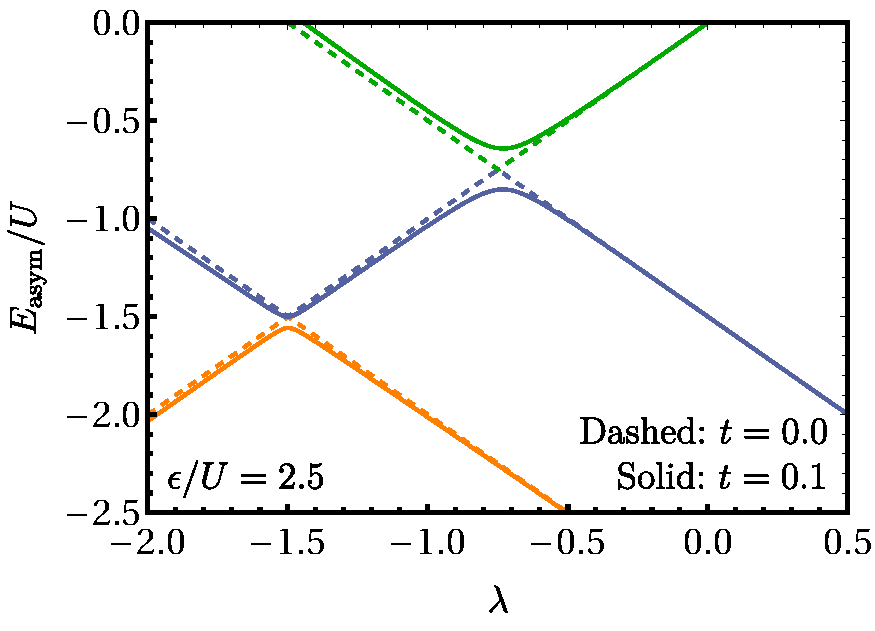
\includegraphics[height=0.75\textwidth]{rmp_cp}	
		\subcaption{\label{subfig:rmp_cp}}
    \end{subfigure}
    %
    \begin{subfigure}{0.32\textwidth}
	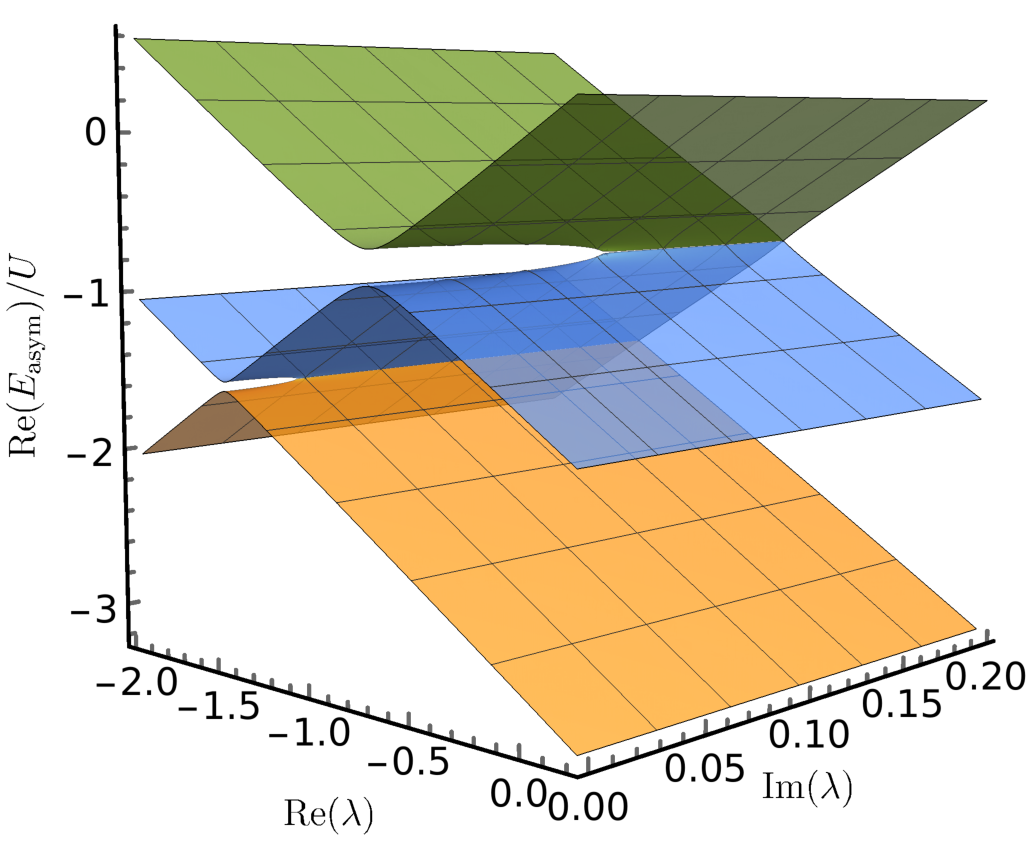
\includegraphics[height=0.75\textwidth]{rmp_cp_surf}
		\subcaption{\label{subfig:rmp_cp_surf}}
    \end{subfigure}
    %
    \begin{subfigure}{0.32\textwidth}
	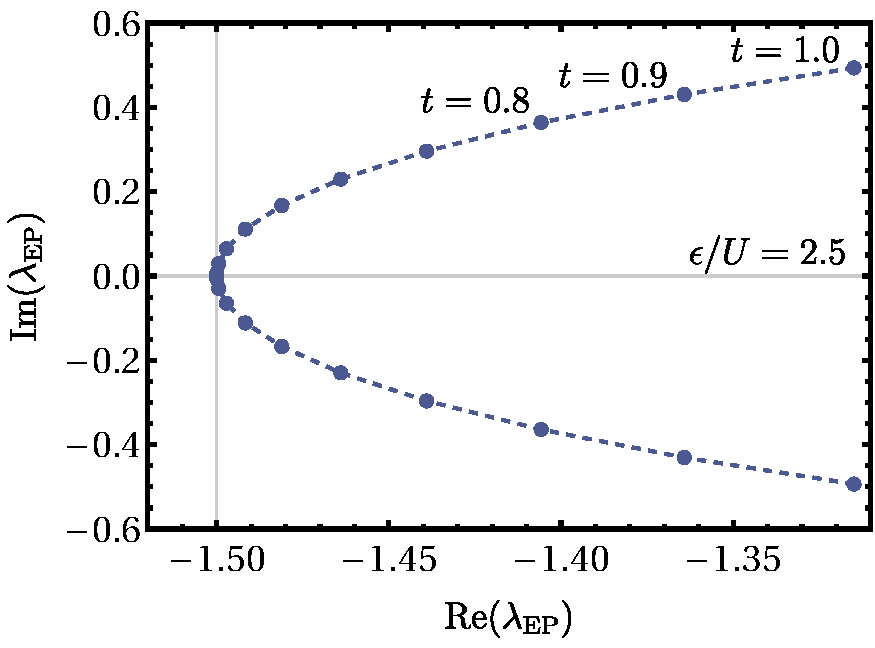
\includegraphics[height=0.75\textwidth]{rmp_ep_to_cp}	
		\subcaption{\label{subfig:rmp_ep_to_cp}}
    \end{subfigure}
	\caption{%
		RMP critical point using the asymmetric Hubbard dimer with $\epsilon = 2.5 U$.
		(\subref{subfig:rmp_cp}) Exact critical points with $t=0$ occur on the negative real $\lambda$ axis (dashed).
		(\subref{subfig:rmp_cp_surf}) Modelling a finite basis using $t=0.1$ yields complex-conjugate EPs close to the
		real axis, giving a sharp avoided crossing on the real axis (solid).
		(\subref{subfig:rmp_ep_to_cp}) Convergence of the ground-state EP onto the real axis in the \trash{exact} limit $t \to 0$.
	\label{fig:RMP_cp}}
\end{figure*}
%------------------------------------------------------------------%

% INTRODUCING THE MODEL
The simplified site basis of the Hubbard dimer makes explicilty modelling the ionisation continuum impossible.
Instead, we can use an asymmetric version of the Hubbard dimer \cite{Carrascal_2015,Carrascal_2018} 
where we consider one of the sites as a ``ghost atom'' that acts as a 
destination for ionised electrons being originally localised on the other site.
To mathematically model this scenario in this asymmetric Hubbard dimer, we introduce a one-electron potential $-\epsilon$ on the left site to 
represent the attraction between the electrons and the model ``atomic'' nucleus [see Eq.~\eqref{eq:H_FCI}], where we define $\epsilon > 0$.
The reference Slater determinant for a doubly-occupied atom can be represented using RHF
orbitals [see Eq.~\eqref{eq:RHF_orbs}] with $\theta_{\alpha}^{\text{RHF}} = \theta_{\beta}^{\text{RHF}} = 0$, 
which corresponds to strictly localising the two electrons on the left site.
%and energy
%\begin{equation}
%   E_\text{HF}(0, 0) = \frac{1}{2} (2 U - 4 \epsilon).
%\end{equation}
With this representation, the parametrised asymmetric RMP Hamiltonian becomes
\begin{widetext}
\begin{equation}
\label{eq:H_asym}
\bH_\text{asym}\qty(\lambda) = 
\begin{pmatrix}
    2(U-\epsilon) - \lambda U &	-\lambda t				 &	-\lambda t	            &	0	        \\
    -\lambda t				  &	(U-\epsilon) - \lambda U &	0		                &	-\lambda t	\\
    -\lambda t				  &	0			             &	(U-\epsilon) -\lambda U	&	-\lambda t	\\
    0 				          &	-\lambda t 	 			 &	-\lambda t              &	\lambda U	\\
\end{pmatrix}.
\end{equation}
\end{widetext}

% DERIVING BEHAVIOUR OF THE CRITICAL SITE
For the ghost site to perfectly represent ionised electrons, the hopping term between the two sites must vanish (\ie, $t=0$).
This limit corresponds to the dissociative regime in the asymmetric Hubbard dimer as discussed in Ref.~\onlinecite{Carrascal_2018}, 
and the RMP energies become
\begin{subequations}
\begin{align}
    E_{-} &= 2(U - \epsilon) - \lambda U,
    \\
    E_{\text{S}} &= (U - \epsilon) - \lambda U,
    \\ 
    E_{+} &= U \lambda,
\end{align}
\end{subequations}
as shown in Fig.~\ref{subfig:rmp_cp} (dashed lines).
The RMP critical point then corresponds to the intersection $E_{-} = E_{+}$, giving the critical $\lambda$ value
\begin{equation}
    \lc = 1 - \frac{\epsilon}{U}. 
\end{equation}
Clearly the radius of convergence $\rc = \abs{\lc}$ is controlled directly by the ratio $\epsilon / U$, 
with a convergent RMP series occurring for $\epsilon > 2 U$.
The on-site repulsion $U$ controls the strength of the HF potential localised around the ``atomic site'', with a
stronger repulsion encouraging the electrons to be ionised at a less negative value of $\lambda$. 
Large $U$ can be physically interpreted as strong electron repulsion effects in electron dense molecules. 
In contrast, smaller $\epsilon$ gives a weaker attraction to the atomic site, 
representing strong screening of the nuclear attraction by core and valence electrons, 
and again a less negative $\lambda$ is required for ionisation to occur.
Both of these factors are common in atoms on the right-hand side of the periodic table, \eg\ \ce{F},
\ce{O}, \ce{Ne}.
Molecules containing these atoms are therefore often class $\beta$ systems with
a divergent RMP series due to the MP critical point. \cite{Goodson_2004,Sergeev_2006} 

% EXACT VERSUS APPROXIMATE
The critical point in the exact case $t=0$ lies on the negative real $\lambda$ axis (Fig.~\ref{subfig:rmp_cp}: dashed lines), 
mirroring the behaviour of a quantum phase transition.\cite{Kais_2006}
However, in practical calculations performed with a finite basis set, the critical point is modelled as a cluster
of branch points close to the real axis.
The use of a finite basis can be modelled in the asymmetric dimer by making the second site a less
idealised destination for the ionised electrons with a non-zero (yet small) hopping term $t$.
Taking the value $t=0.1$ (Fig.~\ref{subfig:rmp_cp}: solid lines), the critical point becomes a
sharp avoided crossing with a complex-conjugate pair of EPs close to the real axis (Fig.~\ref{subfig:rmp_cp_surf}).
In the limit $t \to 0$, these EPs approach the real axis (Fig.~\ref{subfig:rmp_ep_to_cp}),
mirroring Sergeev's discussion on finite basis
set representations of the MP critical point.\cite{Sergeev_2006}

%------------------------------------------------------------------%
% Figure on the UMP critical point
%------------------------------------------------------------------%
\begin{figure*}[t]
	\begin{subfigure}{0.32\textwidth}
        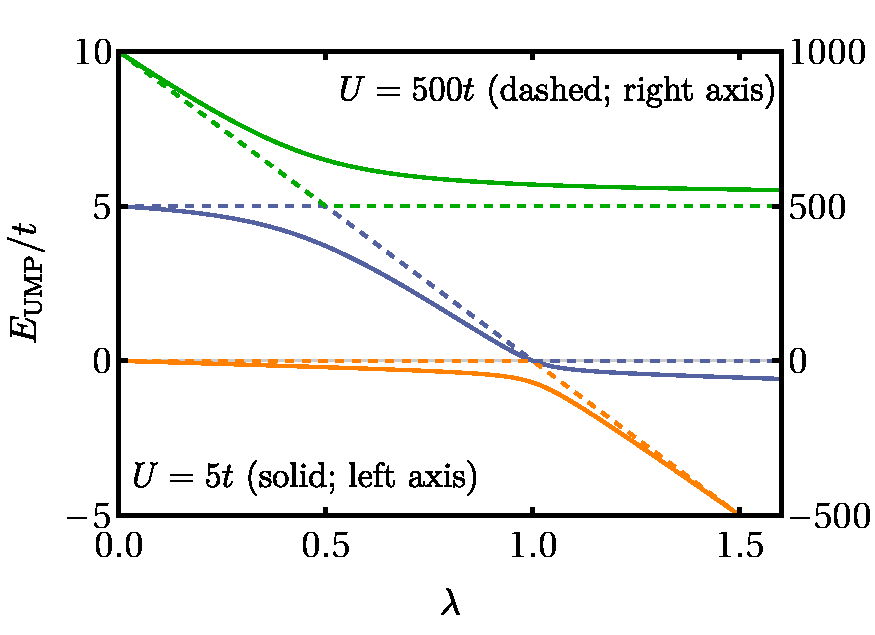
\includegraphics[height=0.75\textwidth,trim={0pt 5pt -10pt 15pt},clip]{ump_cp}	
		\subcaption{\label{subfig:ump_cp}}
    \end{subfigure}
    %
    \begin{subfigure}{0.32\textwidth}
	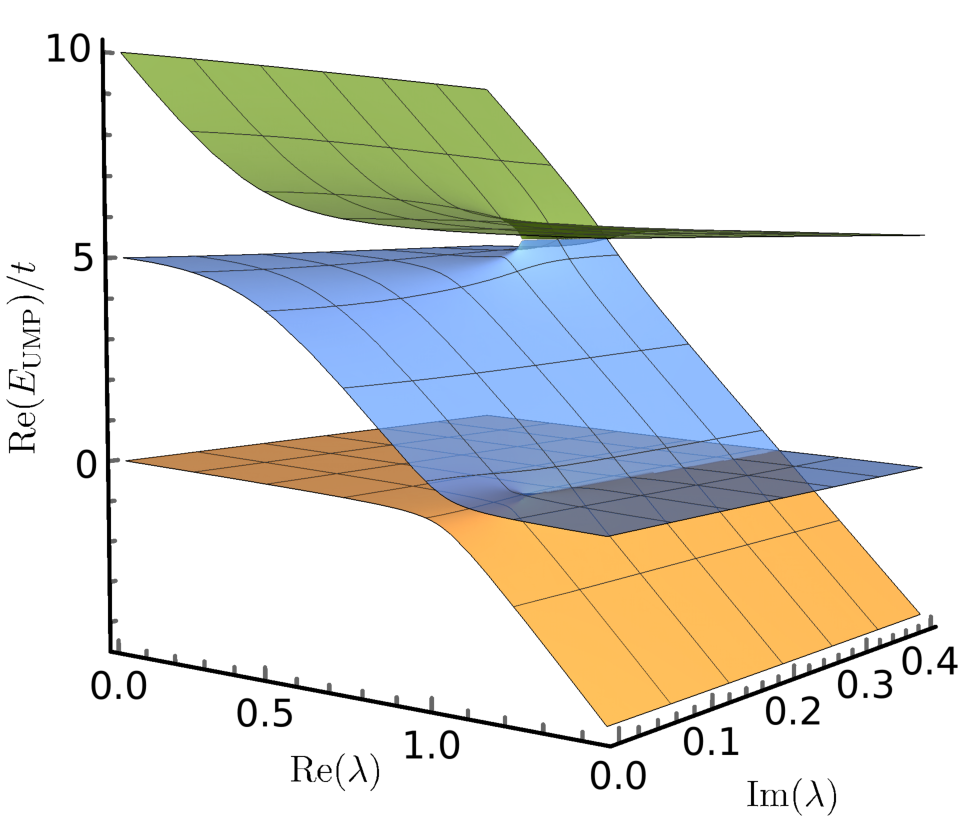
\includegraphics[height=0.75\textwidth]{ump_cp_surf}
		\subcaption{\label{subfig:ump_cp_surf}}
    \end{subfigure}
    %
    \begin{subfigure}{0.32\textwidth}
	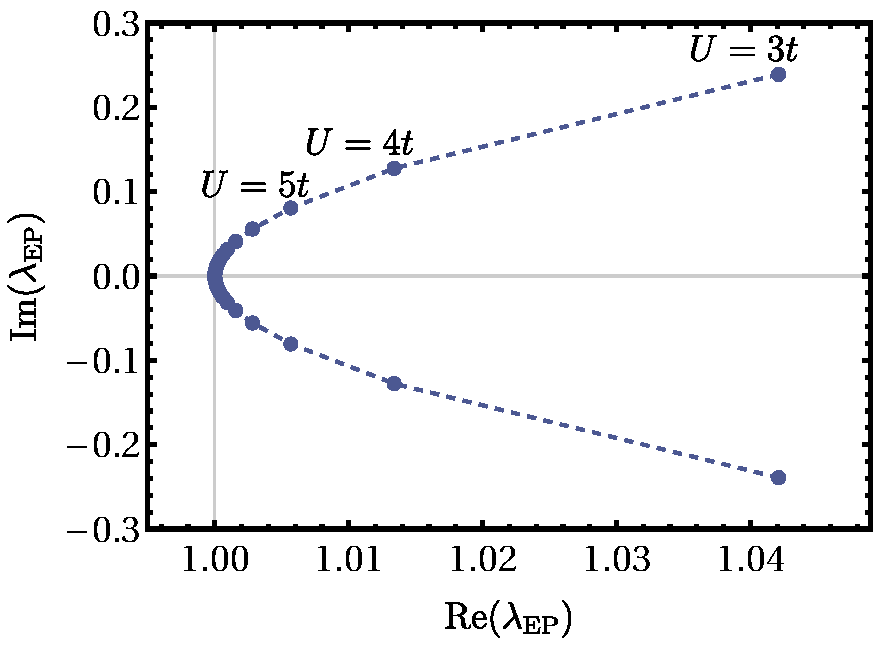
\includegraphics[height=0.75\textwidth]{ump_ep_to_cp}	
		\subcaption{\label{subfig:ump_ep_to_cp}}
    \end{subfigure}
%    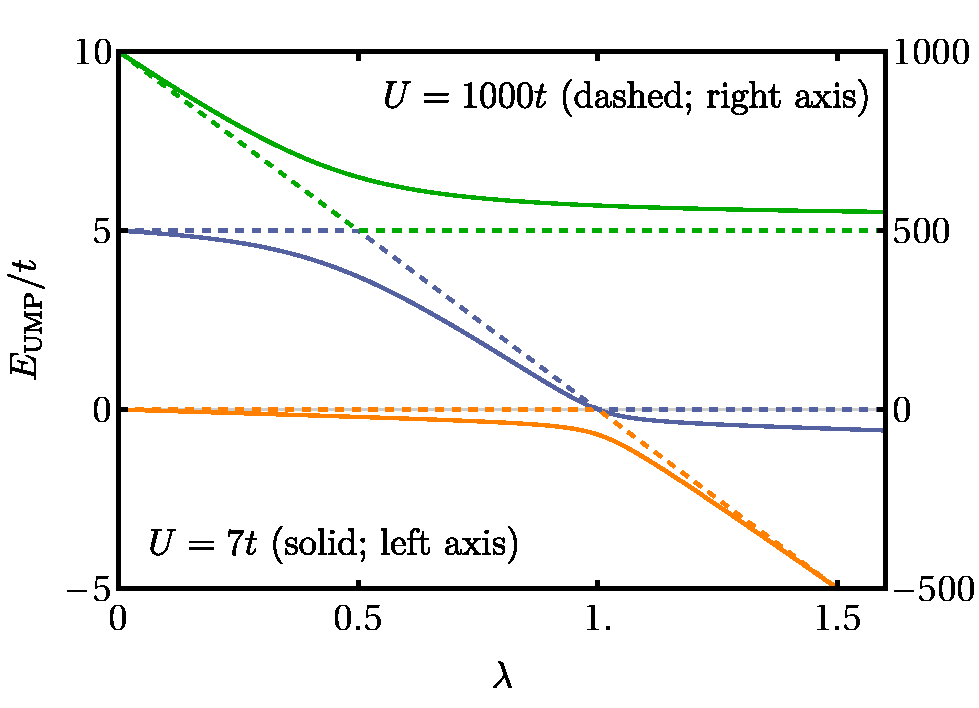
\includegraphics[height=0.65\textwidth,trim={0pt 5pt 0pt 15pt}, clip]{ump_critical_point}
\caption{%
    The UMP ground-state EP \titou{in the symmetric Hubbard dimer} becomes a critical point in the strong correlation limit (\ie, large $U/t$).
    (\subref{subfig:ump_cp}) As $U/t$ increases, the avoided crossing on the real $\lambda$ axis
    becomes increasingly sharp.
    (\subref{subfig:ump_cp_surf}) Complex energy surfaces for $U = 5t$.
    (\subref{subfig:ump_ep_to_cp}) Convergence of the EPs at $\lep$ onto the real axis for $U/t \to \infty$.
    %mirrors the formation of the RMP critical point and other QPTs in the complete basis set limit.
\label{fig:UMP_cp}}

\end{figure*}
%------------------------------------------------------------------%

% RELATIONSHIP BETWEEN QPT AND UMP
Returning to the symmetric Hubbard dimer, we showed in Sec.~\ref{sec:spin_cont} that the slow
convergence of the strongly correlated UMP series
was due to a complex-conjugate pair of EPs just outside the radius of convergence.
These EPs have positive real components and small imaginary components (see Fig.~\ref{fig:UMP}), suggesting a potential 
connection to MP critical points and QPTs (see Sec.~\ref{sec:MP_critical_point}).
For $\lambda>1$, the HF potential becomes an attractive component in Stillinger's 
Hamiltonian displayed in Eq.~\eqref{eq:HamiltonianStillinger}, while the explicit electron-electron interaction
becomes increasingly repulsive.
Closed--shell critical points along the positive real $\lambda$ axis then represent 
points where the two-electron repulsion overcomes the attractive HF potential 
and a single electron dissociates from the molecule (see Ref.~\onlinecite{Sergeev_2006})

In contrast, symmetry-breaking in the UMP reference creates different HF potentials for the spin-up and spin-down electrons.
Consider one of the two reference UHF solutions where the spin-up and spin-down electrons are localised on the left and right sites respectively. 
The spin-up HF potential will then be a repulsive interaction from the spin-down electron 
density that is centred around the right site (and vice-versa).
As $\lambda$ becomes greater than 1 and the HF potentials become attractive, there will be a sudden
driving force for the electrons to swap sites.
This swapping process can also be represented as a double excitation, and thus an avoided crossing will occur
for $\lambda \geq 1$ (Fig.~\ref{subfig:ump_cp}).
While this appears to be an avoided crossing between the ground and first-excited state, 
the presence of an earlier excited-state avoided crossing means that the first-excited state qualitatively 
represents the reference double excitation for $\lambda > 1/2$ (see Fig.~\ref{subfig:ump_cp}).

% SHARPNESS AND QPT
The ``sharpness'' of the avoided crossing is controlled by the correlation strength $U/t$.
For small $U/t$, the HF potentials will be weak and the electrons will delocalise over the two sites,
both in the UHF reference and as $\lambda$ increases.
This delocalisation dampens the electron swapping process and leads to a ``shallow'' avoided crossing
that corresponds to EPs with non-zero imaginary components (solid lines in Fig.~\ref{subfig:ump_cp}).
As $U/t$ becomes larger, the HF potentials become stronger and the on-site repulsion dominates the hopping
term to make electron delocalisation less favourable.
In other words, the electrons localise on individual sites to form a Wigner crystal.
These effects create a stronger driving force for the electrons to swap sites until eventually this swapping
occurs exactly at $\lambda = 1$.
In this limit, the ground-state EPs approach the real axis (Fig.~\ref{subfig:ump_ep_to_cp}) and the avoided 
crossing creates a gradient discontinuity in the ground-state energy (dashed lines in Fig.~\ref{subfig:ump_cp}).
We therefore find that, in the strong correlation limit, the symmetry-broken ground-state EP becomes
a new type of MP critical point and represents a QPT as the perturbation parameter $\lambda$ is varied.
Furthermore, this argument explains why the dominant UMP singularity lies so close, but always outside, the 
radius of convergence (see Fig.~\ref{fig:RadConv}).

%%%%%%%%%%%%%%%%%%%%%%%%%%%%%%%%%%%%%
\section{Resummation Methods}
\label{sec:Resummation}
%%%%%%%%%%%%%%%%%%%%%%%%%%%%%%%%%%%%%

%As frequently claimed by Carl Bender, 
\hugh{It is frequently stated that}
\textit{``the most stupid thing that one can do with a series is to sum it.''}
Nonetheless, quantum chemists are basically doing exactly this on a daily basis.
\hugh{As we have seen throughout this review, the MP series can often show erratic, 
slow, or divergent behaviour.
In these cases, estimating the correlation energy by simply summing successive
low-order terms is almost guaranteed to fail.}
Here, we discuss alternative tools that can be used to sum slowly convergent or divergent series.
\hugh{These so-called ``resummation'' techniques} form a vast field of research and thus we will
provide details for only the most relevant methods.
We refer the interested reader to more specialised reviews for additional information.% 
\cite{Goodson_2011,Goodson_2019}


%==========================================%
\subsection{Pad\'e Approximant}
%==========================================%
\hugh{The failure of a Taylor series for correctly modelling the MP energy function $E(\lambda)$ 
arises because one is trying to model a complicated function containing branch points and
singularities} using a simple polynomial of finite order.
A truncated Taylor series just does not have enough flexibility to do the job properly.
Alternatively, the description of complex energy functions can be significantly improved
by introducing Pad\'e approximants, \cite{Pade_1892} and related techniques. \cite{BakerBook,BenderBook}

\hugh{A Pad\'e approximant can be considered as the best approximation of a function by a 
rational function of given order.}
More specifically, a $[d_A/d_B]$ Pad\'e approximant is defined as 
\begin{equation}
	\label{eq:PadeApp}
	E_{[d_A/d_B]}(\lambda) = \frac{A(\lambda)}{B(\lambda)} 
    = \frac{\sum_{k=0}^{d_A} a_k\, \lambda^k}{1 + \sum_{k=1}^{d_B} b_k\, \lambda^k},
\end{equation}
where the coefficients of the polynomials $A(\lambda)$ and $B(\lambda)$ are determined by collecting terms for each power of $\lambda$.
Pad\'e approximants are extremely useful in many areas of physics and chemistry \cite{Loos_2013,Pavlyukh_2017,Tarantino_2019,Gluzman_2020} as they can model poles, which appears at the locations of the roots of $B(\lambda)$. 
However, they are unable to model functions with square-root branch points (which are ubiquitous in the singularity structure of a typical perturbative treatment) and more complicated functional forms appearing at critical points (where the nature of the solution undergoes a sudden transition).
\hugh{Despite this limitation, the successive diagonal Pad\'e approximants (\ie, $d_A = d_B $) 
often define a convergent perturbation series in cases where the Taylor series expansion diverges.}

Figure \ref{fig:PadeRMP} illustrates the improvement provided by diagonal Pad\'e approximants compared to the usual Taylor expansion in cases where the RMP series of the Hubbard dimer converges ($U/t = 3.5$) and diverges ($U/t = 4.5$).
More quantitatively, Table \ref{tab:PadeRMP} gathers estimates of the RMP ground-state energy at $\lambda = 1$ provided by various truncated Taylor series and Pad\'e approximants for these two values of the ratio $U/t$.
While the truncated Taylor series converges laboriously to the exact energy as the truncation degree increases at $U/t = 3.5$, the Pad\'e approximants yield much more accurate results.
\hugh{Furthermore, the Pad\'e approximants provide a rather good estimate of the radius of convergence of the RMP series.}
For $U/t = 4.5$, the Taylor series expansion performs worse (and eventually diverges),
while the Pad\'e approximants still offer relaitively accurate energies even outside the radius of convergence of the RMP series.

\hugh{%
We can expect that the singularity structure of the UMP energy will be much more challenging to model properly as the UMP energy function contains three connected branches (see Figs.~\ref{subfig:UMP_3} and \ref{subfig:UMP_7}).
Figure~\ref{fig:QuadUMP} and Table~\ref{tab:QuadUMP} indicate that this is indeed the case. 
However, with sufficiently high degree polynomials, one obtains
accurate estimates of both the radius of convergence and the ground-state energy at $\lambda = 1$,
even in cases where the convergence of the UMP series is incredibly slow 
(see Fig.~\ref{subfig:UMP_cvg}).
In Figure \ref{fig:QuadUMP}, it becomes clear that the Pad\'e approximants are trying to model
the square root branch point that lies close to $\lambda = 1$ by placing a pole on the real axis
(for [3/3]) or with a very small imaginary component (for [4/4]).
The proximity of these poles to the radius of convergence means that any error in the Pad\'e 
functional form becomes magnified in the estimate of energy at $\lambda = 1$.
}

\begin{table}
	\caption{RMP ground-state energy estimate at $\lambda = 1$ provided by various truncated Taylor series and Pad\'e approximants at $U/t = 3.5$ and $4.5$.
	We also report the estimate of the radius of convergence $r_c$ provided by the diagonal Pad\'e approximants.
	\label{tab:PadeRMP}}
	\begin{ruledtabular}
		\begin{tabular}{lccccc}
						&			&	\mc{2}{c}{$r_c$}			&	\mc{2}{c}{$E_{-}(\lambda = 1)$}			\\
																		\cline{3-4} \cline{5-6}
			Method		&	degree	&	$U/t = 3.5$	&	$U/t = 4.5$	&	$U/t = 3.5$	&	$U/t = 4.5$	\\
			\hline
			Taylor		&	2		&			&			&	$-1.01563$	&	$-1.01563$	\\
						&	3		&			&			&	$-1.01563$	&	$-1.01563$	\\
						&	4		&			&			&	$-0.86908$	&	$-0.61517$	\\
						&	5		&			&			&	$-0.86908$	&	$-0.61517$	\\
						&	6		&			&			&	$-0.92518$	&	$-0.86858$	\\
			Pad\'e		&	[1/1]	&	$2.29$	&	$1.78$	&	$-1.61111$	&	$-2.64286$	\\
						&	[2/2]	&	$2.29$	&	$1.78$	&	$-0.82124$	&	$-0.48446$	\\
						&	[3/3]	&	$1.73$	&	$1.34$	&	$-0.91995$	&	$-0.81929$	\\
						&	[4/4]	&	$1.47$	&	$1.14$	&	$-0.90579$	&	$-0.74866$	\\
						&	[5/5]	&	$1.35$	&	$1.05$	&	$-0.90778$	&	$-0.76277$	\\
			\hline
			Exact		&			&	$1.14$	&	$0.89$	&	$-0.90754$	&	$-0.76040$	\\
		\end{tabular}
	\end{ruledtabular}
\end{table}

%%%%%%%%%%%%%%%%%
\begin{figure*}
    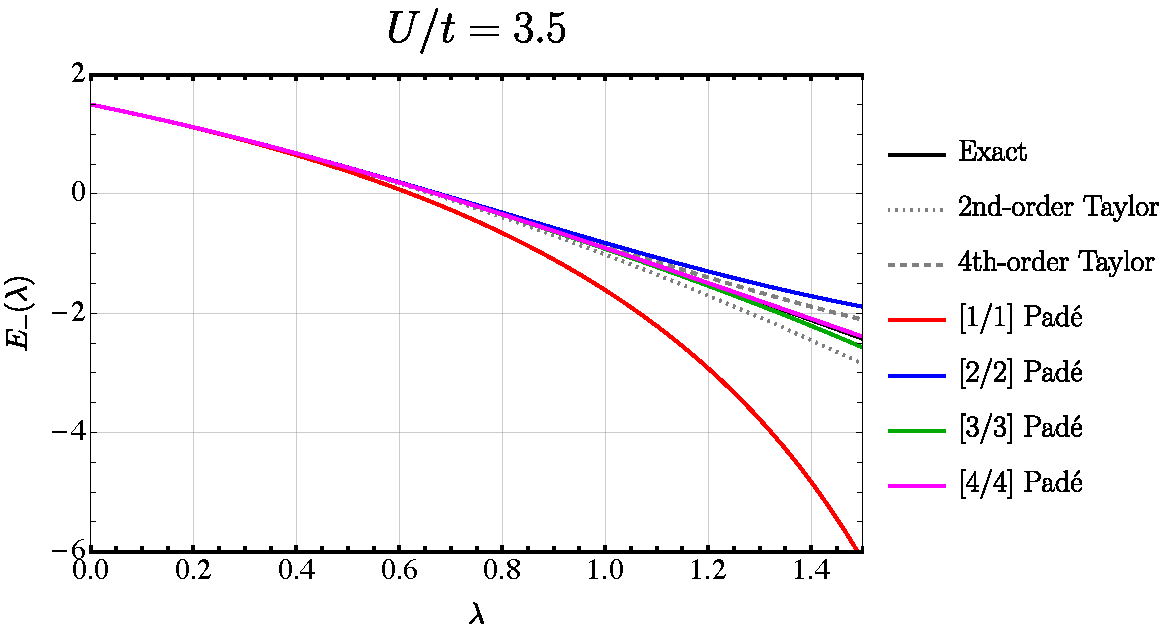
\includegraphics[height=0.23\textheight]{PadeRMP35}
    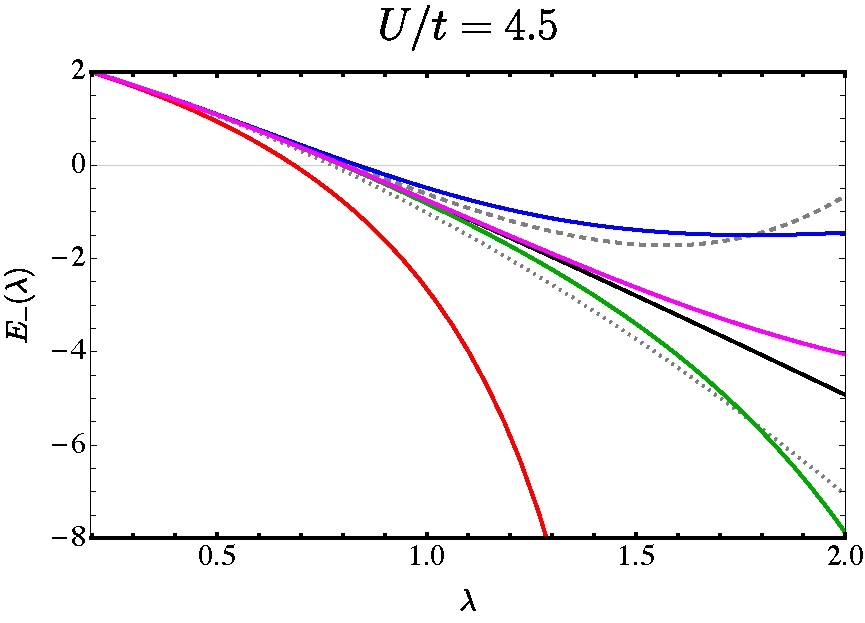
\includegraphics[height=0.23\textheight]{PadeRMP45}
    \caption{\label{fig:PadeRMP}
    RMP ground-state energy as a function of $\lambda$ obtained using various resummation techniques at $U/t = 3.5$ (left) and $U/t = 4.5$ (right).}
\end{figure*}
%%%%%%%%%%%%%%%%%

%==========================================%
\subsection{Quadratic Approximant}
%==========================================%
Quadratic approximants \hugh{are designed} to model the singularity structure of the energy function $E(\lambda)$ via a generalised version of the square-root singularity expression \cite{Mayer_1985,Goodson_2011,Goodson_2019}
\begin{equation}
	\label{eq:QuadApp}
	E(\lambda) = \frac{1}{2 Q(\lambda)} \qty[ P(\lambda) \pm \sqrt{P^2(\lambda) - 4 Q(\lambda) R(\lambda)} ]
\end{equation}
with the polynomials 
\begin{align}
	\label{eq:PQR}
	P(\lambda) & = \sum_{k=0}^{d_P} p_k \lambda^k,
	&
	Q(\lambda) & = \sum_{k=0}^{d_Q} q_k \lambda^k, 
	&
	R(\lambda) & = \sum_{k=0}^{d_R} r_k \lambda^k 
\end{align}
defined such that $d_P + d_Q + d_R = n - 1$, and $n$ is the truncation order of the Taylor series of $E(\lambda)$.
Recasting Eq.~\eqref{eq:QuadApp} as a second-order expression in $E(\lambda)$, \ie,
\begin{equation}
	Q(\lambda) E^2(\lambda) - P(\lambda) E(\lambda) + R(\lambda) \sim \order*{\lambda^{n+1}}
\end{equation}
and substituting $E(\lambda$) by its $n$th-order expansion and the polynomials by their respective expressions \eqref{eq:PQR} yields $n+1$ linear equations for the coefficients $p_k$, $q_k$, and $r_k$ (where we are free to assume that $q_0 = 1$).
A quadratic approximant, characterised by the label $[d_P/d_Q,d_R]$, generates, by construction, $n_\text{bp} = \max(2d_p,d_q+d_r)$ branch points at the roots of the polynomial $P^2(\lambda) - 4 Q(\lambda) R(\lambda)$.
The diagonal sequence of quadratic approximant, \ie, $[0/0,0]$, $[1/0,0]$, $[1/0,1]$, $[1/1,1]$, $[2/1,1]$, is of particular interest.
However, by construction, a quadratic approximant has only two branches, which hampering the faithful description of more complicated singularity structures.
As shown in Ref.~\onlinecite{Goodson_2000a}, quadratic approximants provide convergent results in the most divergent cases considered by Olsen and collaborators \cite{Christiansen_1996,Olsen_1996} and Leininger \etal \cite{Leininger_2000}

For the RMP series of the Hubbard dimer, the $[0/0,0]$ and $[1/0,0]$ quadratic approximant are quite poor approximations, but the $[1/0,1]$ version perfectly models the RMP energy function by predicting a single pair of EPs at $\lambda_\text{EP} = \pm i 4t/U$.
This is expected from the form of the RMP energy [see Eq.~\eqref{eq:E0MP}], which matches the ideal target for quadratic approximants.

%%%%%%%%%%%%%%%%%
\begin{figure}
    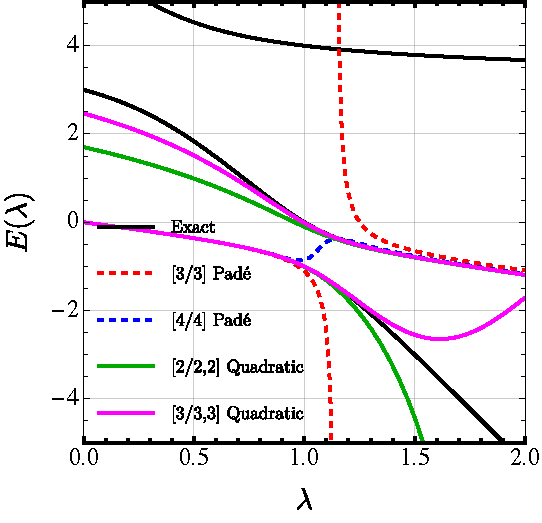
\includegraphics[width=\linewidth]{QuadUMP}
    \caption{\label{fig:QuadUMP}
    UMP energies as a function of $\lambda$ obtained using various resummation techniques at $U/t = 3$.}
\end{figure}
%%%%%%%%%%%%%%%%%

\begin{table}
	\caption{Estimate of the radius of convergence $r_c$ of the UMP energy function provided by various resummation techniques at $U/t = 3$ and $7$.
	The truncation degree of the Taylor expansion $n$ of $E(\lambda)$ and the number of branch points $n_\text{bp} = \max(2d_p,d_q+d_r)$ generated by the quadratic approximants are also reported.
	\label{tab:QuadUMP}}
	\begin{ruledtabular}
		\begin{tabular}{lccccccc}
						&			&			&					&	\mc{2}{c}{$r_c$}	&	\mc{2}{c}{$E_{-}(\lambda)$}			\\
																		\cline{5-6}\cline{7-8}
			\mc{2}{c}{Method}		&	$n$		&	$n_\text{bp}$	&	$U/t = 3$	&	$U/t = 7$	&	$U/t = 3$	&	$U/t = 7$	\\
			\hline
			Pad\'e		&	[1/1]	&	2		&					&	$9.000$		&	$49.00$		&	$-0.75000$	&	$-0.29167$	\\
                        &	[2/2]	&	4		&					&	$0.974$		&	$1.003$		&	$\hphantom{-}0.75000$	&	$-17.9375$	\\
			         	&	[3/3]	&	6		&					&	$1.141$		&	$1.004$		&	$-1.10896$	&	$-1.49856$	\\
						&	[4/4]	&	8		&					&	$1.068$		&	$1.003$		&	$-0.85396$	&	$-0.33596$	\\
						&	[5/5]	&	10		&					&	$1.122$		&	$1.004$		&	$-0.97254$	&	$-0.35513$	\\
			Quadratic	&	[2/1,2]	&	6		&	4				&	$1.086$		&	$1.003$		&	$-1.01009$	&	$-0.53472$	\\
						&	[2/2,2]	&	7		&	4				&	$1.082$		&	$1.003$		&	$-1.00553$	&	$-0.53463$	\\
						&	[3/2,2]	&	8		&	6				&	$1.082$		&	$1.001$		&	$-1.00568$	&	$-0.52473$	\\
						&	[3/2,3]	&	9		&	6				&	$1.071$		&	$1.002$		&	$-0.99973$	&	$-0.53102$	\\
						&	[3/3,3]	&	10		&	6				&	$1.071$		&	$1.002$		&	$-0.99966$	&	$-0.53103$	\\
			\hline
			Exact		&			&			&					&	$1.069$		&	$1.002$		&	$-1.00000$	&	$-0.53113$	\\
		\end{tabular}
	\end{ruledtabular}
\end{table}
\hugh{On the other hand, the greater flexibility of the quadratic approximants provides a significantly
improved model of the UMP energy in comparison to the Pad\' approximants or Taylor series.
In particular, the quadratic approximants provide an effect model for the avoided crossings 
(Fig.~\ref{fig:QuadUMP}) and a far better estimate for the location of the branch point singularities.
Furthermore, they provide remarkably accurate estimates of the ground-state energy at $\lambda = 1$, 
as shown in Table~\ref{tab:QuadUMP}}

However, as a note of caution, Ref.~\onlinecite{Goodson_2019} suggests that low-order 
quadratic approximants can struggle to correctly model the singularity structure when 
the energy function has poles in both the positive and negative half-planes. 
In such a scenario, the quadratic approximant will tend to place its branch points in-between, potentially introducing singularities quite close to the origin.
The remedy for this problem involves applying a suitable transformation of the complex plane (such as a bilinear conformal mapping) which leaves the points at $\lambda = 0$ and $\lambda = 1$ unchanged. \cite{Feenberg_1956}


%==========================================%
\subsection{Shanks Transformation}
%==========================================%

While the Pad\'e and quadratic approximants can yield a convergent series representation
in cases where the standard MP series diverges, there is no guarantee that the rate of convergence
will be fast enough for low-order approximations to be useful.
However, these low-order partial sums or approximants often contain a remarkable amount of information
that can be used to extract further information about the exact result.
The Shanks transformation presents one approach for extracting this information
and accelerating the rate of convergence of a sequence.\cite{Shanks_1955}

Consider the partial sums $S_N$ defined from the truncated summation of an infinite series
\begin{equation}
    S_N = \sum_{k=0}^{N} a_k.
\end{equation}
If the series converges, then the partial sums will tend to the exact result in the limit $N\rightarrow \infty$.
The Shanks transformation attempts to generate increasingly accurate estimates of the
exact result by defining a new series as
\begin{equation}
    T(S_N) = \frac{S_{N+1} S_{N-1} - S_{N}^2}{S_{N+1} + S_{N-1} - 2 S_{N}}.
\end{equation}
This series can converge faster than the original partial sums and can thus provide greater
accuracy using only the first few terms in the series.


%==========================================%
\subsection{Analytic continuation}
%==========================================%

Recently, Mih\'alka \textit{et al.} studied the partitioning effect on the convergence properties of Rayleigh-Schr\"odinger perturbation theory by considering the MP and the EN partitioning as well as an alternative partitioning \cite{Mihalka_2017a} (see also Ref.~\onlinecite{Surjan_2000}).
Taking as an example (in particular) the water molecule at equilibrium and at stretched geometries, they could estimate the radius of convergence via a quadratic Pad\'e approximant and convert divergent perturbation expansions to convergent ones in some cases thanks to a judicious choice of the level shift parameter.
In a subsequent study by the same group, \cite{Mihalka_2017b} they use analytic continuation techniques to resum divergent MP series \cite{Goodson_2011} taking again as an example the water molecule in a stretched geometry.
In a nutshell, their idea consists in calculating the energy of the system for several values of $\lambda$ for which the MP series is rapidly convergent (\ie, for $\abs{\lambda} < r_c$), and to extrapolate the final energy to the physical system at $\lambda = 1$ via a polynomial- or Pad\'e-based fit. 
However, the choice of the functional form of the fit remains a subtle task.
This technique was first generalised by using complex scaling parameters and applying analytic continuation by solving the Laplace equation, \cite{Surjan_2018} and then further improved thanks to Cauchy's integral formula \cite{Mihalka_2019}
\begin{equation}
	\label{eq:Cauchy}
	\frac{1}{2\pi i} \oint_{\gamma} \frac{E(\lambda)}{\lambda - a} = E(a),
\end{equation}
which states that the value of the energy can be computed at $\lambda=a$ inside the complex contour $\gamma$ only by the knowledge of its values on the same contour.
Their method consists in refining self-consistently the values of $E(\lambda)$ computed on a contour going through the physical point at $\lambda = 1$ and encloses points of the ``trusted'' region (where the MP series is convergent). The shape of this contour is arbitrary but no singularities are allowed inside the contour to ensure $E(\lambda)$ is analytic. 
When the values of $E(\lambda)$ on the so-called contour are converged, Cauchy's integrals formula \eqref{eq:Cauchy} is invoked to compute the values at $E(\lambda=1)$ which corresponds to the final estimate of the FCI energy.
The authors illustrate this protocol on the dissociation curve of \ce{LiH} and the stretched water molecule showing encouraging results. \cite{Mihalka_2019} 

%%%%%%%%%%%%%%%%%%%%
\section{Conclusion}
%%%%%%%%%%%%%%%%%%%%

In order to model accurately chemical systems, one must choose, in an ever growing zoo of methods, which computational protocol is adapted to the system of interest.
This choice can be, moreover, motivated by the type of properties that one is interested in.
That means that one must understand the strengths and weaknesses of each method, \ie, why one method might fail in some cases and work beautifully in others. 
We have seen that for methods relying on perturbation theory, their successes and failures are directly connected to the position of singularities in the complex plane, known as exceptional points.

After a short presentation of the fundamental notions of quantum chemistry in the complex plane, such as the mean-field Hartree--Fock approximation and Rayleigh--Schr\"odinger perturbation theory, we have provided an exhaustive historical overview of the various research activities that have been performed on the physics of singularities with a particular focus on M{\o}ller--Plesset perturbation theory. 
Seminal contributions from various research groups around the world have evidenced highly oscillatory, slowly convergent, or catastrophically divergent behaviour of the restricted and/or unrestricted MP perturbation series.\cite{Laidig_1985,Knowles_1985,Handy_1985,Gill_1986,Laidig_1987,Nobes_1987,Gill_1988,Gill_1988a,Lepetit_1988} 

Later, these erratic behaviours were investigated and rationalised in terms of avoided crossings and singularities in the complex plane. 
In that regard, it is worth highlighting the key contribution of Cremer and He who proposed a classification of the types of convergence: \cite{Cremer_1996} ``class A'' systems that exhibit monotonic convergence, and ``class B'' systems for which convergence is erratic after initial oscillations. 
Further insights were brought thanks to a series of papers by Olsen and coworkers \cite{Christiansen_1996,Olsen_1996,Olsen_2000,Olsen_2019} where they employ a two-state model to dissect the various convergence behaviours of Hermitian and non-Hermitian perturbation series.
Building on the careful mathematical analysis of Stillinger who showed that the mathematical origin behind the divergent series with odd-even sign alternation is due to a dominant singularity on the negative real $\lambda$ axis, \cite{Stillinger_2000} Sergeev and Goodson proposed a more refined singularity classification: $\alpha$ singularities which have ``large'' imaginary parts, and $\beta$ singularities which have very small imaginary parts. \cite{Goodson_2000a,Goodson_2000b,Goodson_2004,Sergeev_2005,Sergeev_2006}
We have further highlighted that these so-called $\beta$ singularities are connected to quantum phase transitions and symmetry breaking.

Finally, we have discussed several resummation techniques, such as Pad\'e and quadratic approximants, that can be used to improve energy estimates for both convergent and divergent series.
However, it is worth mentioning that the construction of these approximants requires high-order MP coefficients which are quite expensive to compute in practice.

Most of the concepts reviewed in the present manuscript has been illustrated on the symmetric (or asymmetric in one occasion) Hubbard dimer at half-filling.
Although extremely simple, this clearly illustrates the obvious versatility of the Hubbard model to understand perturbation theory as well as other concepts such as Kohn-Sham density-functional theory (DFT), \cite{Carrascal_2015} linear-response theory, \cite{Carrascal_2018} many-body perturbation theory, \cite{Romaniello_2009,Romaniello_2012,DiSabatino_2015,Tarantino_2017}, DFT for ensembles, \cite{Deur_2017,Deur_2018,Senjean_2018,Sagredo_2018,Fromager_2020} and many others.
We believe that the Hubbard dimer could then be used for further developments around perturbation theory.

As a concluding remark and from a broader point of view, the present work shows that our understanding of the singularity structure of the energy is still incomplete.
Yet, we hope that the present contribution will open new perspectives for the understanding of the physics of exceptional points in electronic structure theory.

%%%%%%%%%%%%%%%%%%%%%%%%
\begin{acknowledgements}
%%%%%%%%%%%%%%%%%%%%%%%%
This project has received funding from the European Research Council (ERC) under the European Union's Horizon 2020 research and innovation programme (Grant agreement No.~863481).
HGAB gratefully acknowledges New College, Oxford for funding through the Astor Junior Research Fellowship.
%%%%%%%%%%%%%%%%%%%%%%
\end{acknowledgements}
%%%%%%%%%%%%%%%%%%%%%%

%%%%%%%%%%%%%%%%%%%%%%
\bibliography{EPAWTFT}
%%%%%%%%%%%%%%%%%%%%%%

\end{document}
